%\documentclass[a4paper]{article}
\documentclass[a4paper,oneside]{memoir}
\usepackage[hscale=0.76,vscale=0.76]{geometry}
\setlength{\parindent}{0.0cm}
\setlength{\parskip}{1.4ex}
\usepackage{graphicx}
\usepackage{proof}
\usepackage{fancyvrb}
%%% Japanese
\usepackage{fontspec,xltxtra,xunicode}
\usepackage{indentfirst}

% freely available M+ fonts
\setmainfont[Mapping=tex-text]{M+ 2p regular}
\setsansfont[Mapping=tex-text]{M+ 2c regular}
\setmonofont[Mapping=tex-text]{M+ 2m medium}
%\setmainfont[Mapping=tex-text]{メイリオ}
%\setsansfont[Mapping=tex-text]{Hiragino Kaku Gothic ProN W3}
%\setmonofont[Mapping=tex-text]{Osaka-Mono}
%\setjamonofont{Osaka-Mono}
\XeTeXlinebreaklocale "ja"
\XeTeXlinebreakskip=0em plus 0.1em minus 0.01em
\XeTeXlinebreakpenalty=0
\renewcommand{\baselinestretch}{1.4}
\settowidth{\parindent}{あ}
%%%%
\usepackage{dcolumn,hhline,colortbl}
\usepackage[table]{xcolor}
%%%%% 色付表
\newcolumntype{G}{%
  >{\columncolor[gray]{0.9}}c}
\newcolumntype{O}{%
  >{\columncolor{orange}}c}
\newcolumntype{M}{%
  >{\columncolor{green}}c}
\newcolumntype{Y}{%
  >{\columncolor{yellow}}c}
\newcolumntype{C}{%
  >{\columncolor{cyan}}c}
%%%% hyperref
%\usepackage[dvipdfm,colorlinks=true,linkcolor=blue]{hyperref} 
\usepackage[colorlinks=true,linkcolor=blue]{hyperref} 
%%%% numbering
%%% ToC down to susubsections
\settocdepth{subsubsection}
%%% Numbering down to sections
\setsecnumdepth{subsection}
%%% 名前定義を適当に
\def\figurename{{図}}
\def\tablename{表}
\def\contentsname{目次}
\def\listfigurename{図目次}
\def\listtablename{表目次}
\def\refname{参考文献}
\def\bibname{参考文献}
\def\indexname{索引}
\def\appendixname{付録}
%%%%%%%%%% Verbatim
\DefineVerbatimEnvironment%
{simplev}{Verbatim}
{fontsize=\small}
\DefineVerbatimEnvironment%
{examplev}{Verbatim}
{frame=leftline,fontsize=\small}
%%%%%%%%%%
\definecolor{shadecolor}{gray}{0.9}
\newenvironment{vvtm}%
{\parskip=0pt\lineskip=0pt\begin{center}\begin{minipage}{0.8\textwidth}\begin{snugshade}}%
  {\end{snugshade}\end{minipage}\end{center}}
%\includeonly{appendix}
%%%%%%%%%%
\begin{document}
\headstyles{default}
\tightlists
\midsloppy
\raggedbottom
\chapterstyle{ell}
%%%%%%%%
\frontmatter
\pagestyle{empty}
% 表紙 %%%%%%%%%%%%%%%%%%%%%%%%%%%%%%%%%%%%%%%%%%%%%%%%%%%%%
\title{\textbf{PigNose 使用手引}\\ver 1.0 \\ --\textit{Draft}--}
\author{澤田 寿実\\
  info@cafeobj.org}
\date{}
\maketitle
  \begin{center}
    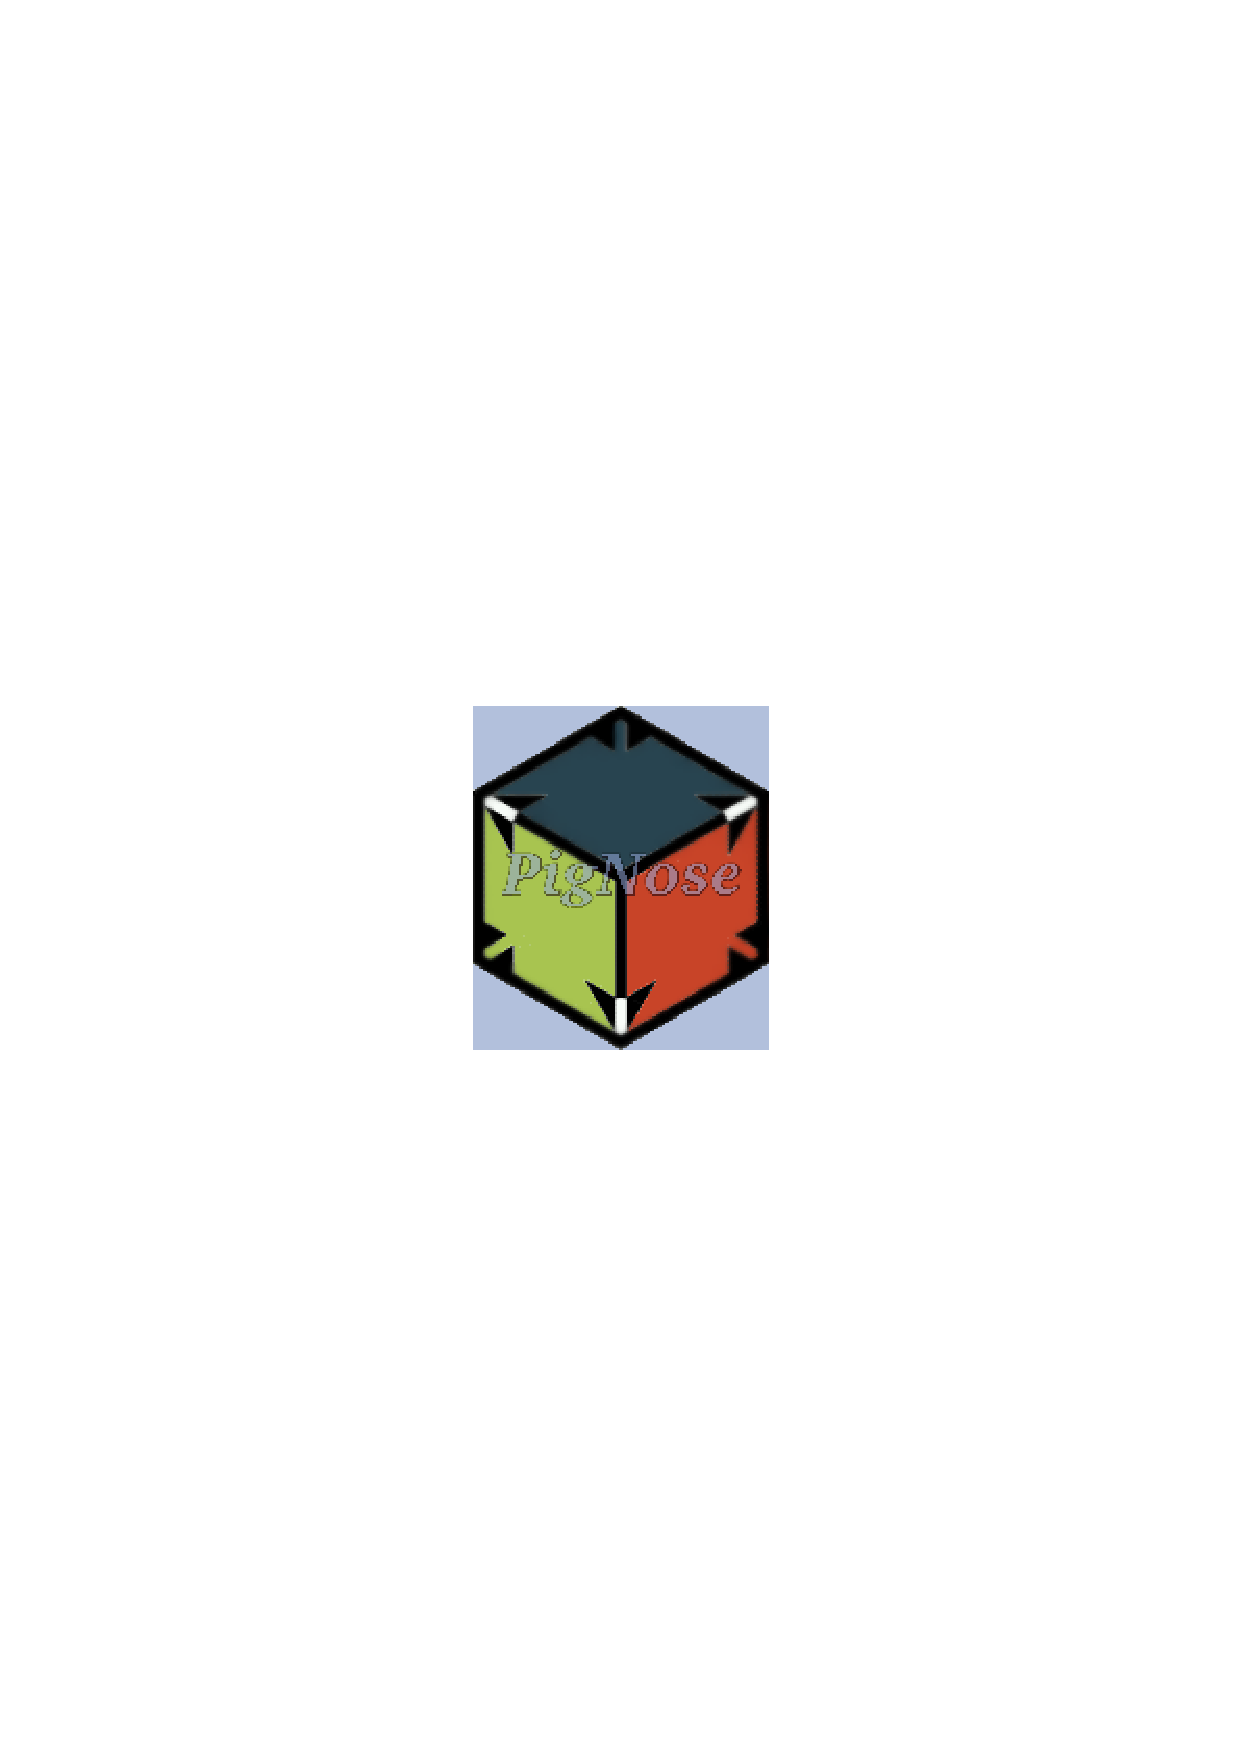
\includegraphics[scale=0.5]{pignose.pdf}
  \end{center}
\thispagestyle{empty}
\newpage
% 構成 %%%%%%%%%%%%%%%%%%%%%%%%%%%%%%%%%%%%%%%%%%%%%%%%%%%%%
\section*{はじめに}
本書は, CafeOBJ 言語で書かれた仕様のための自動定理証明システム
PigNose の利用手引である. 
システムは SRA版 CafeOBJ インタプリタ\footnote{今の所, CafeOBJ 言語のイ
  ンタプリタはこれしか存在しない. システムの入手先については第
  ~\ref{sec:distribution}節を参照されたい.} 
を拡張したものになっている. 
従って, これを用いるには CafeOBJ インタプリタの使用法
についても知っておく必要がある. 本書では, PigNose 特有のコマンドについて
のみ説明するので, 必要に応じて CafeOBJ インタプリタのマニュアル\footnote{CafeOBJ インタプリタのマニュアルは
   \url{http://cafeobj.org/download/} からダウンロード
   出来る}. 
を参照されたい.
また, ここでは CafeOBJ 言語についての説明も行わない. 本書では, CafeOBJ
言語については既知のものと仮定している. CafeOBJ 言語についての解説は, 文
献\cite{CafeRep}を参照して頂きたい. 
% PigNose は resolution 原理を用いた反駁法によって定理証明を行うシステムで
% あるが, これについての解説も行わない. 
% 必要に応じて, 参考文献 \cite{chang-lee} 等を参照して頂きたい.  

% \section*{本書の構成}

本文は4部構成でPigNoseシステムの使用法が説明されている.
第I部でシステムのインストール法を述べ, 第II部で反駁エンジン,
第III部で詳細化検証, 第IV部で安全性モデル検査について説明する.

\section*{バグレポート/提案}

システムの不具合に関する報告や, 改善提案等に関する
連絡は, 電子メイルで \texttt{info@cafeobj.org} まで頂きたい.

\newpage
% 目次 %%%%%%%%%%%%%%%%%%%%%%%%%%%%%%%%%%%%%%%%%%%%%%%%%%%%%
% \doparttoc
\tableofcontents
\newpage
%\listoffigures
%\newpage
\pagenumbering{arabic}
\mainmatter
% 本文 %%%%%%%%%%%%%%%%%%%%%%%%%%%%%%%%%%%%%%%%%%%%%%%%%%%%%
%\part*{PigNose�V�X�e���̊T�v}

{\LARGE\textbf{PigNose�V�X�e���̊T�v}}
\label{sec:system-overall}
%\addcontentsline{toc}{part}{PigNose�V�X�e���̊T�v}
\vspace*{1cm}

PigNose �̎�ȖړI�́CCafeOBJ����ŏ����ꂽ�d�l���^����ꂽ�Ƃ�, 
\begin{itemize}
\item ���̎d�l�ŕ\�����ꂽ�V�X�e����, �^����ꂽ������
  ��������邩�ǂ��������؂���.
\end{itemize}
�Ƃ������̂ł���. 
���ɏd�v�Ǝv���鎟�̂Q�_�ɂ‚��Ă͂��ꂼ��ɓ������ꂽ�@�\��
�񋟂���Ă���F
\begin{itemize}
\item[(1)] ���ꂪ(�ʂɗp�ӂ��ꂽ)�d�l $M$ �Ɛ����I�ł��邱��($M$ �̑S��
  �̌������^����ꂽ�d�l�ł��������邱��)�𔻒肷��.

\item[(2)] ���̎d�l�ɂ���ĕ\���ꂽ�V�X�e����, ���鎖�O�����𖞑����Ă�
  ��Ȃ��, �����ĕs�����ȏ�ԂɂȂ�����\�����Ȃ��U�������邱�Ƃ��Ȃ�,
  �Ƃ������S��(safety)��(�����I��)�������s������.
\end{itemize}
�{���ł�(1)��\textbf{�ڍ׉�����}, (2)��\textbf{���S�����f������
  }�ƌĂ�. 

�������������邽��, PigNose �͎��̂悤�Ȋg����CafeOBJ�ɑ΂�
�Ď{�����F
\begin{itemize}
\item[(a)] ���\�[�g�̈�K�q��_�����ɂ��L�q���”\�Ƃ�, 
\item[(b)] ���̏�ł̎����藝�ؖ��@�\��񋟂���.
\end{itemize}
(a)����CafeOBJ����ɑ΂���g���ƌ��鎖���o���邪, PigNose�̖{���I�ȈӐ}
�͂����ɂ͖���, ���p�҂̕ւ�}���Ă̎��ł���. ����, �]����CafeOBJ�����
�����ꂽ�d�l�ɑ΂���, �Ȃ��ύX���{��������PigNose�V�X�e���̋@�\�𗘗p
���邱�Ƃ��ł���. ��K�q��_���̓�����, ���̕\���\�͂̍����ɂ����̂ł�
��, CafeOBJ����̃��W���[�����@�\��p����, PigNose�ɂ��g���Ə�����
CafeOBJ ����ɂ��d�l�L�q�𖾊m�ɐ؂蕪���邱�Ƃ��o����.
�]���� PigNose �� CafeOBJ �C���^�v���^�ɐV���ɓ������ꂽ�c�[���Ƃ݂Ȃ���
�悢. 

���(b)���̒藝�ؖ��@�\��, ��Ɍ��y�����ڍ׉����؂ƈ��S�����f�������ŕK
�v�ƂȂ�藝�ؖ���Ƃ����s������̂ł���. �������܂�(���\�[�g)��K�q��_
���n��ΏۂƂ�, resolution ����\cite{chang-lee}���x�[�X�Ƃ���, �����G��
�W���Ƃ��Ď�������Ă���. 
�����G���W���͓Ɨ������藝�ؖ��V�X�e���Ƃ��ė��p���鎖���”\�ł���.
�{�G���W����p���鎖�ɂ����, ���p�҂� CafeOBJ �ŋL�q���ꂽ�d�l�ɑ΂���
, ���܂��܂Ȍ������ȕւɎ��s���邱�Ƃ��o����. 
�����G���W�����̂�, ���ɗǂ��m��ꂽ�����藝�ؖ���
\textsc{Otter}~\cite{otter}���Q�l�ɂ��Ă��̋@�\���݌v���ꂽ.
�G���W���̒��j�����̋@�\�́C��{�I�� \textsc{Otter} �̂���̃T�u�Z�b�g��
�Ȃ��Ă��邪, ���\�[�g�_��������, CafeOBJ �ŏ����ꂽ�d�l�ɑ΂���, ���̕�
�X�������邱�ƂȂ��ɒ藝�ؖ����s����悤�ɔz������Ă���.

�ȏ�q�ׂ������𔽉f��, PigNose �͎���3�‚̃T�u�V�X�e������\������Ă�
��F
\begin{enumerate}
\item �����G���W��
\item �ڍ׉����؃V�X�e��
\item ���f�������V�X�e��
\end{enumerate}

�ڍ׉�����/���f�������e�V�X�e�����g�p�����, �����G���W���Ɋւ��Ă̗���
������Ɣ��ɖ��ɗ���. �{���ł͍ŏ��ɔ����G���W���ɂ‚��Ă̎g�p������q
��, �‚��ŏڍ׉�����, ���f�������Ƃ������e�V�X�e���̎g�p���@���������.

%%% Local Variables: 
%%% mode: latex
%%% TeX-master: t
%%% End: 

%% part II
\part{���󥹥ȡ�����ˡ}

\section{�����ƥ��׵�}
\label{sec:system-req}

\subsection{�ץ�åȥե�����}
\label{sec:platform}

���ڿ��������ƥ�� CafeOBJ ���󥿥ץ꥿�ξ�˹��ۤ���륷���ƥ�Ǥ���,
CafeOBJ ���󥿥ץ꥿����Ư����Ķ��Ǥ���Ф褤. CafeOBJ���󥿥ץ꥿���Τ�
Common Lisp ������Ѥ��Ƶ��Ҥ���Ƥ��뤿��, ����Ū�� Common Lisp
���󥿥ץ꥿����Ư����Ķ��Ǥ�������̵꤬����, �ºݤˤ�ư���
�ץ�åȥե�����˰�¸������ʬ������. 
�ʤ������ƥ�μ¹ԴĶ��ˤ����Ƥ�, �١����Ȥ��� Common Lisp ��
��Ư����ɬ�פΤ��뤳�Ȥ����դ��줿��. 

���ߤν�, �ʲ��ν����ϤǤ�
ư���ǧ����Ƥ���(ɽ\ref{tab:platform}�˷Ǥ�����Ư�ץ�åȥե������
�����ʥꥹ�ȤǤϤʤ�. �ܺ٤ˤĤ��Ƥϳơ��ν����Ϥλ����򻲾Ȥ��줿��).

\begin{table}[htbp]
  \begin{center}
    \begin{tabular}{|l|l|}\hline
      Common Lisp ������ & ��Ư�ץ�åȥե�����\\\hline\hline
      GCL(version 2.3�ʾ�) 
      & i386 Linux, BSD \\
      & Sun Sparc, Sun OS 5(gcc) \\\hline
      Allegro Common Lisp (ver5.0�ʾ�) & Linux \\
      & Windows95/98 \\\hline
      CMU CommonLisp & Sparc Slaris \\
      & i386 Linux \\\hline
      CLISP & i386 Linux \\\hline
    \end{tabular}
    \caption{CafeOBJ ���󥿥ץ꥿�β�Ư�Ķ�}
    \label{tab:platform}
  \end{center}
\end{table}

�嵭����Ӥ����㳰�� Common Lisp �����ϤˤĤ��Ƥξ����, 
\textbf{The Association of Lisp Users} �Υۡ���ڡ���
\verb+http://www.lisp.org+ ����Υ�󥯤򤿤ɤ����, �ưפ�����Ǥ���.

\subsection{�����ƥ�꥽����}
���󥹥ȡ���ˤ����äƤ�, �١����Ȥ��� Common Lisp �����Ϥ˰�¸����
���Ѥ���ǥ������ΰ��¥����ɬ���̤��ۤʤ�. 

����Ū�˼¥���� 128Mbyte �ʾ�Ǥ��뤳�Ȥ�˾�ޤ���.
�ǥ����ȥ�ӥ塼������ UNIX TAR �����Υ��������֥ե������ gzip 
�ǸǤ᤿�����Ǥ���, ���Υ��������� 700K �Х��ȤǤ���.
�����Ÿ�������, ��3.8Mbyte �Υǥ������ΰ����Ѥ���.
���󥹥ȡ���˺ݤ��Ƥ�, �ɤ� Common Lisp �����Ϥ���Ѥ��뤫�ˤ�ä�
�Ȥ���ǥ��������̤��礭���ۤʤ뤬, ��20Mbyte ���٤ζ����ΰ褬
���ݤ���Ƥ��뤳�Ȥ�˾�ޤ���. 

\section{���󥹥ȡ�����ˡ}

\subsection{�ǥ����ȥ�ӥ塼��������}
�����ƥ�ϥ������������󶡤����.
����� Unix �Υơ��ץ��������ַ���(TAR)�ե������ gzip �ˤ�äƸǤ᤿
�ե�����η��Ǥ���. ����ˤ� CafeOBJ ���󥿥ץ꥿���ΤΥ�������ޤޤ�
�Ƥ���. ���ۤϥ��󥿡��ͥåȾ�� ftp �����Ȥ����������Ȥ���������
����, ���ߤν�ʲ��Υ����Ȥ������������ɲ�ǽ�Ǥ���.

\begin{verbatim}
  ftp://ftp.sra.co.jp/pub/lang/CafeOBJ/cafeobj-1.4.4PigNoseXXXX.tar.gz
\end{verbatim}

������, \verb+XXXX+ �ϥС�������ֹ�Ǥ���. 
20001ǯ2��ߤκǿ��С�������ֹ�� \verb+0.95c+ �Ǥ���, �������ä�
�嵭�Υե�����̾��
\begin{verbatim}
    cafeobj-1.4.4PigNose0.95c.tar.gz
\end{verbatim}
�Ǥ���. 
 
�ʹߤǤ�, ���Υե������ñ��\textbf{�ǥ����ȥ�ӥ塼�����}�ȸƤ�.
�����Ÿ������� \verb+cafeobj-1.4.4PigNose0.95c+ �Ȥ����ǥ��쥯�ȥ�
����������, ���β��˥��󥹥ȡ����ɬ�פʥ������ե������饤�֥����
���֤����. �㤨�� Unix ��Ǥϼ��Τ褦�ˤ���Ÿ�����롧
\begin{verbatim}
 % gunzip -c cafeobj-1.4.4PigNose0.95c.tar.gz | tar xvf -
\end{verbatim}
�ʲ�Ÿ�����ƺ������줿�ǥ��쥯�ȥ�β��ǥ��󥹥ȡ����Ȥ�
�¹Ԥ�����Ȥʤ�. 

\subsection{Unix/Linux ��ǤΥ��󥹥ȡ�����ˡ}
Unix (Linux) ��ǤΥ��󥹥ȡ���ϰʲ��Τ褦�˹Ԥ�.
\begin{enumerate}
\item �ǥ����ȥ�ӥ塼������Ÿ�������ǥ��쥯�ȥ�ذ�ư����.
\begin{verbatim}
  % cd cafeobj-1.4.4PigNose0.95c
\end{verbatim}
\item ���Ѥ��� Common Lisp �����Ϥ�, ���󥹥ȡ�����Υǥ��쥯�ȥ��
  �����Ԥ�. ����ˤϥǥ����ȥ�ӥ塼�����˴ޤޤ�Ƥ���
  \texttt{configure} ���ޥ�ɤ򼡤Τ褦�ˤ��Ƶ�ư���뤳�Ȥˤ�äƹԤ�:
{\small
\begin{verbatim}
  % ./configure [-with-lisp=<Lisp�����ϻ���>] [-prefix=<���󥹥ȡ�����>]
\end{verbatim}
}
  ������, $<$Lisp�����ϻ���$>$ �ϥ١����Ȥ��ƻ��Ѥ��� Common Lisp ������
  �λ���Ǥ���, �ʲ��Τ�Τ��椫����ꤹ�롧
  \begin{enumerate}
    \item[(1)]\texttt{gcl} --- GCL
    \item[(2)]\texttt{acl} --- Allegro Common Lisp (ver 5.01 �ʲ�)
    \item[(3)]\texttt{acl6} --- Allegro Common Lisp (ver 6.0 �ʾ�)
    \item[(4)]\texttt{cmu-sparc} -- CMU Common Lisp, Sparc Sun OS
    \item[(5)]\texttt{cmu-pc} --- CMU Common Lisp, i386 �ޥ���
    \item[(6)]\texttt{clisp} --- CLISP
  \end{enumerate}
  �ä˻����Ԥ�ʤ���� gcl ���ǥե���Ȥ����򤵤��.

  $<$���󥹥ȡ�����$>$ ��, �����ƥ�򥤥󥹥ȡ��뤹��ǥ��쥯�ȥ��
  �ѥ�̾����ꤹ���ΤǤ���. �ä˻��̵꤬�����,
  �ǥե���Ȥ� \texttt{/usr/local} �����󥹥ȡ�����Ȥʤ�. 

\item make ���ޥ�ɤˤ�ä�, �����ƥ�ι���/���󥹥ȡ����Ԥ�.
\begin{verbatim}
  % make bigpink
  % make install-bigpink
\end{verbatim}
  �ǽ�� make ���ޥ�ɤ�ȯ���ˤ�ä�, �����ƥ�Υ���ѥ��뤬
  �Ԥ��, ���� make ���ޥ�ɤ�ȯ���ˤ�ä�, �����ƥब�����
  �ǥ��쥯�ȥ�˥��󥹥ȡ��뤵���.
\end{enumerate}

\subsection{Windows95/96 ��ǤΥ��󥹥ȡ�����ˡ}

���ߤν�, Windows95/98 ��� CafeOBJ ���󥿥ץ꥿��,
Allegro Common Lisp (ver 5.0 �ʾ�) -- ACL -- ���ꤷ�����󥹥ȡ����礬
�Ѱդ���Ƥ���. ����ϰʲ��μ��ˤ�롧
\begin{enumerate}
\item ACL ��ư����.
\item ACL ���󥿥ץ꥿�Υȥåץ�٥륳�ޥ�� \texttt{:cd} ���Ѥ���
  �ǥ����ȥ�ӥ塼������Ÿ�������ǥ��쥯�ȥ�˰�ư���롧
\item 
\end{enumerate}

%%% Local Variables: 
%%% mode: latex
%%% TeX-master: t
%%% End: 

\part{���͸��ڥ����ƥม�����͡����}
\label{sec:spec-test}

���͸��ڥ����ƥ��, ɽ\ref{tab:system-functions}��
��ǽ��1��(���ʹ֤μͤμ�ư������ǽ)��, 
��3��(�ܺٲ����ڵ�ǽ)���б����륵�֥����ƥ�Ǥ���.
�ʹߤǤ�, �����2�Ĥε�ǽ���դ��Ƹ������ͤȸ�����̤򼨤�.
�ܥ����ƥ��ȿ�������ƥ���󶡤��뵡ǽ��ե�˻��Ѥ��Ƥ��뤿��,
�����ǹԤ������������ˤ�����븡����, ȿ�������ƥ���Ф���
����Ū�ʸ����ΰ�̣�⤢��.

\section{���ʹ֤μͤμ�ư������ǽ}
\label{sec:sigmatch}
�ܾϤǤ�, ���ʹ֤μͤμ�ư������ǽ�˴ؤ��븡�����ܤȤ��η��, 
�ʤ�Ӥ˳Ƹ������ܤζ���Ū�����Ƥ��դ��ƽҤ٤�.

\subsection{��������}
\label{sec:sigmatch-test-item}
�������ܤϼ����̤�Ǥ��롧
\begin{enumerate}
\item ñ��ʼͤ�����\\
  ��ǽ�ʼͤ���Ĥ˸¤�����ˤĤ���, �������ͤ���������뤳�Ȥ򸡺�����.

\Item ʣ���μͤ����� \\
  ��ǽ�ʼͤ���Ĥ˸¤��ʤ����ˤĤ���, ��ǽ�ʼͤ���������
  �������򸡺�����.

\item �ͤ������Ǥ��ʤ����\\
  ��ǽ�ʼͤ���Ĥ�ʤ����ˤĤ���, �ͤ���������ʤ����Ȥ�
  ��������.

\end{enumerate}

\subsection{������̰���}
\label{sec:sigmatch-test-res-all}
��\ref{sec:sigmatch-test-item}��Ǽ������Ƹ������ܤ��Ф���
������̤�ɽ\ref{tab:sigmatch-test-res}�˼���. 

\begin{table}[htbp]
  \begin{center}
    \begin{tabular}[h]{|l|c|c|}\hline
      �������� & ��� & �������ֹ� \\\hline
      ñ��ʼͤ����� & �� & \ref{sec:mono-view} \\
      ʣ���μͤ����� & �� & \ref{sec:multi-view} \\
      �ͤ������Ǥ��ʤ���� & �� & \ref{sec:null-view} \\\hline
    \end{tabular}
    \caption{���ʹ֤μͤμ�ư������ǽ�������}
    \label{tab:sigmatch-test-res}
  \end{center}
\end{table}

\subsection{ñ��ʼͤ�����}
\label{sec:mono-view}
\subsubsection{��������}

\begin{enumerate}
\item ���ͼ͹����Υ١����Ȥ���⥸�塼����Ф���
  ñ��μͤΤߤ������Ǥ���⥸�塼��Ȥδ֤�,
  ���ͼͤμ�ư������ǽ(���ޥ�� \verb:sigmatch:)��
  ��ư��, ñ��μͤ��������������ɤ����򸡺�����.
\item �������줿�ͤ�, ͽ�ۤ�����Τ�Ʊ����ʪ�Ǥ��뤫�ɤ�����,
  ���ޥ�� \verb:show view: ���Ѥ����������줿�ͤ�
  ������, ���Ƥ�Ĵ�٤뤳�Ȥˤ�äƹԤ�.
\end{enumerate}

����Ū�ʥƥ������Ƥ�ͽ�۷�̤ˤĤ��Ƥ�, ����򻲾Ȥ��줿��.

\subsubsection{�ƥ��ȥǡ����ȼ��}
\label{sec:sigmatch-mono-data}

\begin{enumerate}
\item ���˼����褦��, �⥸�塼�뷲�������
  sigmatch ���ޥ�ɤε�ư������ץȤ�,
  �ե����� ``sigmatch-mono.mod'' �˽񤭹���Ǥ���.

{\small
\begin{verbatim}
**>
**> ñ��μͤμ�ư�����ƥ��ȤΤ���Υ⥸�塼�������
**> sigmatch ���ޥ�ɤε�ư
**>

-->
--> �١����Ȥʤ�⥸�塼�� �� CONTAINER
-->

mod* CONTAINER(X :: TRIV) 
{
  *[ Container ]*

  op empty : -> Container
  bop store : Elt Container -> Container
  bop val : Container -> Elt
}

-->
--> �ƥ����оݤΥ⥸�塼�� : BUF
--> 
mod* BUF(X :: TRIV)
{
  *[ Buf ]*
  op init :  -> Buf 
  bop in : Elt Buf -> Buf
  bop val : Buf -> Elt
  bop out : Buf -> Buf
  bop empty? : Buf -> Bool
}

**> sigmatch ��ư
--> sigmatch (CONTAINER) to (BUF)
-->
sigmatch (CONTAINER) to (BUF)

-->
--> �ƥ����оݤΥ⥸�塼�� : CELL
--> 
mod* CELL(X :: TRIV) 
{
  *[ Cell ]*

  op init-cell : -> Cell
  bop put : Elt Cell -> Cell
  bop get : Cell -> Elt
}

**> sigmatch ��ư
--> sigmatch (CONTAINER) to (CELL)
-->
sigmatch (CONTAINER) to (CELL)

-->
--> �ƥ����оݤΥ⥸�塼�� : LIST
--> 
mod* LIST(X :: TRIV)  
{

  *[ List ]*

  op nil : -> List   
  op cons : Elt List -> List {coherent}
  bop car : List -> Elt
  bop cdr : List -> List
}

**> sigmatch ��ư
--> sigmatch (CONTAINER) to (LIST)
-->
sigmatch (CONTAINER) to (LIST)

-->
--> �ƥ����оݤΥ⥸�塼�� : QUEUE
--> 

mod* QUEUE(X :: TRIV) 
{
  *[ Queue ]*
  op empty : -> Queue 
  bop front : Queue -> Elt
  bop enq : Elt Queue -> Queue
  bop deq : Queue -> Queue
}

**> sigmatch ��ư
--> sigmatch (CONTAINER) to (QUEUE)
-->
sigmatch (CONTAINER) to (QUEUE)

-->
--> �ƥ����оݤΥ⥸�塼�� : STACK
--> 

mod* STACK(X :: TRIV) 
{
  *[ Stack ]*
  op empty : -> Stack
  bop top : Stack -> Elt
  bop push : Elt Stack -> Stack
  bop pop : Stack -> Stack
}

**> sigmatch ��ư
--> sigmatch (CONTAINER) to (STACK)
-->
sigmatch (CONTAINER) to (STACK)

**
eof
\end{verbatim}
}
\item �����϶ˤ�ñ��ʥ����˥���Ǥ���, ��ǽ�ʻ��ͼͤϤ�����Ĥ���
  ̵�������ưפ�ʬ����. ��ǽ�ʼͤϼ��ΤȤ���Ǥ��롧
  �ޤ�, ���Ƥξ��ˤĤ���, CONTAINER �α��쥽���� Container ��,
  ���줾���оݤȤ����⥸�塼����������Ƥ���ͣ��α��쥽����
  (�㤨�Х⥸�塼�� BUF �ξ���, Buf)�˼��������Ϥ��Ǥ���.
  �ޤ�, ���ڥ졼�����б��ط��ϲ��˼����褦�ˤʤ�Ϥ��Ǥ���.
  \begin{enumerate}
  \item �⥸�塼�� BUF �ξ�硧
  \begin{verbatim}
    empty ---> init
    val   ---> val
    store ---> in
  \end{verbatim}
  \item �⥸�塼�� CELL �ξ�硧
  \begin{verbatim}
    empty ---> init-cell
    val   ---> get
    store ---> put
  \end{verbatim}  
  \item �⥸�塼�� LIST �ξ�硧
  \begin{verbatim}
    empty ---> nil
    val   ---> car
    store ---> cons
  \end{verbatim}
  \item �⥸�塼�� QUEUE �ξ��:
  \begin{verbatim}
    empty ---> empty
    val   ---> front
    store ---> enq
  \end{verbatim}
  \item �⥸�塼�� STACK �ξ�硧
  \begin{verbatim}
    empty ---> empty
    val   ---> top
    store ---> push
  \end{verbatim}
  \end{enumerate}

\item �������줿���ͼͤ����Ƥ�, �� \verb:sigmatch: �ε�ư�ˤ�ä�
  �����ƥब��������ͤ�̾���򸫤�, ����� \verb:show view: ���ޥ�ɤ�
  �����Ȥ���Ϳ������ˤ�ä�ɽ������.
  ���줬, ��ǽҤ٤���ǽ�ʼͤ�Ʊ�����ɤ�����Ĵ�٤�.
\end{enumerate}

\subsubsection{�¹Է��}
\begin{enumerate}
\item ����(��\ref{sec:sigmatch-mono-data}��)�ǽҤ٤��ƥ��ȥǡ�����
  �񤭹�����ե����� ``sigmatch-mono.mod'' �򥤥󥿥ץ꥿���ɤ߹����.
  ��̤Υ����ϰʲ����̤�Ǥ���.
{\small
  \begin{verbatim}
CafeOBJ> in sigmatch-mono
processing input : ./sigmatch-mono.mod
**> 
**> ñ��μͤμ�ư�����ƥ��ȤΤ���Υ⥸�塼�������
**> sigmatch ���ޥ�ɤε�ư
**> 
--> 
--> �١����Ȥʤ�⥸�塼�� �� CONTAINER
--> 
-- defining module* CONTAINER_*_*....._*
** system failed to prove =*= is a congruence of CONTAINER done.
--> 
--> �ƥ����оݤΥ⥸�塼�� : BUF
--> 
-- defining module* BUF_*_*......._*
** system failed to prove =*= is a congruence of BUF done.
**> sigmatch ��ư
--> sigmatch (CONTAINER) to (BUF)
--> 
(V#1)
--> 
--> �ƥ����оݤΥ⥸�塼�� : CELL
--> 
-- defining module* CELL_*_*....._*
** system failed to prove =*= is a congruence of CELL done.
**> sigmatch ��ư
--> sigmatch (CONTAINER) to (CELL)
--> 
(V#2)
--> 
--> �ƥ����оݤΥ⥸�塼�� : LIST
--> 
-- defining module* LIST_*_*......_*
** system failed to prove =*= is a congruence of LIST done.
**> sigmatch ��ư
--> sigmatch (CONTAINER) to (LIST)
--> 
(V#3)
--> 
--> �ƥ����оݤΥ⥸�塼�� : QUEUE
--> 
-- defining module* QUEUE_*_*......_*
** system failed to prove =*= is a congruence of QUEUE done.
**> sigmatch ��ư
--> sigmatch (CONTAINER) to (QUEUE)
--> 
(V#4)
--> 
--> �ƥ����оݤΥ⥸�塼�� : STACK
--> 
-- defining module* STACK_*_*......_*
** system failed to prove =*= is a congruence of STACK done.
**> sigmatch ��ư
--> sigmatch (CONTAINER) to (STACK)
--> 
(V#5)
  \end{verbatim}
}
  ����򸫤��, ���줾��ˤĤ��Ƥ�����Ĥμͤ���������Ƥ���.
  �����ͽ���̤�Ǥ���.

\item ����, �嵭�η�̥����ƥब���������ͤ�ɽ����, ���Ƥ�
  ��ǧ���뤿���, show view ���ޥ�ɤ��Ѥ��Ƥ��줾���
  �ͤ��������. ��̤ϲ����̤�Ǥ��롧
{\small
  \begin{verbatim}
CafeOBJ> show view V#1
view V#1 from CONTAINER(X) to BUF(X) {sort Elt -> Elt
    hsort Container -> Buf
    hsort ?Container -> ?Buf
    op (Container : -> SortId) -> (Buf : -> SortId)
    op (Elt : -> SortId) -> (Elt : -> SortId)
    op (_=*=_ : Container Container -> Bool) -> (_=*=_ : _ HUniversal _
                                                         _ HUniversal _
                                                         -> 
                                                        Bool)
    op (empty : -> Container) -> (init : -> Buf)
    bop (val : Container -> Elt) -> (val : Buf -> Elt)
    bop (store : Elt Container -> Container) -> (in : Elt Buf
                                                      -> Buf)
 }
CafeOBJ> show view V#2
view V#2 from CONTAINER(X) to CELL(X) {sort Elt -> Elt
    hsort Container -> Cell
    hsort ?Container -> ?Cell
    op (Container : -> SortId) -> (Cell : -> SortId)
    op (Elt : -> SortId) -> (Elt : -> SortId)
    op (_=*=_ : Container Container -> Bool) -> (_=*=_ : _ HUniversal _
                                                         _ HUniversal _
                                                         -> 
                                                        Bool)
    op (empty : -> Container) -> (init-cell : -> Cell)
    bop (val : Container -> Elt) -> (get : Cell -> Elt)
    bop (store : Elt Container -> Container) -> (put : Elt Cell
                                                       -> Cell)
 }
CafeOBJ> show view V#3
view V#3 from CONTAINER(X) to LIST(X) {sort Elt -> Elt
    hsort Container -> List
    hsort ?Container -> ?List
    op (Container : -> SortId) -> (List : -> SortId)
    op (Elt : -> SortId) -> (Elt : -> SortId)
    op (_=*=_ : Container Container -> Bool) -> (_=*=_ : _ HUniversal _
                                                         _ HUniversal _
                                                         -> 
                                                        Bool)
    op (empty : -> Container) -> (nil : -> List)
    bop (val : Container -> Elt) -> (car : List -> Elt)
    bop (store : Elt Container -> Container) -> (cons : Elt List
                                                        -> List)
 }
CafeOBJ> show view V#4
view V#4 from CONTAINER(X) to QUEUE(X) {sort Elt -> Elt
    hsort Container -> Queue
    hsort ?Container -> ?Queue
    op (Container : -> SortId) -> (Queue : -> SortId)
    op (Elt : -> SortId) -> (Elt : -> SortId)
    op (_=*=_ : Container Container -> Bool) -> (_=*=_ : _ HUniversal _
                                                         _ HUniversal _
                                                         -> 
                                                        Bool)
    op (empty : -> Container) -> (empty : -> Queue)
    bop (val : Container -> Elt) -> (front : Queue -> Elt)
    bop (store : Elt Container -> Container) -> (enq : Elt Queue
                                                       -> Queue)
 }
CafeOBJ> show view V#5
view V#5 from CONTAINER(X) to STACK(X) {sort Elt -> Elt
    hsort Container -> Stack
    hsort ?Container -> ?Stack
    op (Container : -> SortId) -> (Stack : -> SortId)
    op (Elt : -> SortId) -> (Elt : -> SortId)
    op (_=*=_ : Container Container -> Bool) -> (_=*=_ : _ HUniversal _
                                                         _ HUniversal _
                                                         -> 
                                                        Bool)
    op (empty : -> Container) -> (empty : -> Stack)
    bop (val : Container -> Elt) -> (top : Stack -> Elt)
    bop (store : Elt Container -> Container) -> (push : Elt Stack
                                                        -> Stack)
 }
  \end{verbatim}
}

  ��̤�ͽ���̤�Ǥ���, ������.
\end{enumerate}

\subsection{ʣ���μͤ�����}
\label{sec:multi-view}
\subsubsection{��������}
\begin{enumerate}
\item ʣ���λ��ͼͤ���������⥸�塼����ȹ礻���Ф���
  sigmatch ���ޥ�ɤ�ư��, ��̤Ȥ���ʣ���μͤ�
  �ºݤ˹�������뤳�Ȥ��ǧ����.
\item �������줿���줾��μͤ�, ���餫�������ꤵ��Ƥ���
  �ͤȰ��פ����Τ��ɤ������ǧ����. 
  ����Ͼ�� sigmatch ���ޥ�ɤμ¹Ԥη������줿
  �ͤ�̾���򻲾Ȥ�, show view ���ޥ�ɤˤ�äƼͤ����Ƥ�
  ����������ˤ�äƹԤ�.
\end{enumerate}

����Ū�ʥƥ������Ƥ�ͽ�۷�̤ˤĤ��Ƥ�, ����ǽҤ٤�.

\subsubsection{�ƥ��ȥǡ����ȼ��}
\label{sec:multi-view-test-data}

\begin{enumerate}
\item ���˼����褦��, �⥸�塼���������� sigmatch ���ޥ�ɤ�
  ��ư������ץȤ�, �ե����� ``sigmatch-mult.mod'' �˽񤭹���Ǥ���.
\begin{verbatim}
**>
**> ʣ���μͤμ�ư�����ƥ��ȤΤ���Υ⥸�塼�������
**> sigmatch ���ޥ�ɤε�ư
**>

-->
--> �١����Ȥʤ�⥸�塼�� �� CONTAINER
-->

mod* CONTAINER(X :: TRIV) 
{
  *[ Container ]*

  op empty : -> Container
  bop store : Elt Container -> Container
  bop val : Container -> Elt
}

-->
--> �ƥ����оݤΥ⥸�塼�� : MTEST
--> 
mod* MTEST(X :: TRIV)
{
  *[ H ]*

  op init : -> H
  bop m1   : H Elt -> H
  bop m2   : Elt H -> H
  bop a1   : H -> Elt
  bop a2   : H -> Elt
}

**> sigmatch ���ޥ�ɤε�ư
--> sigmatch (CONTAINER) to (MTEST)
-->
sigmatch (CONTAINER) to (MTEST)
\end{verbatim}
\item ����򥤥󥿥ץ꥿���ɤ߹���ʣ���� view ����������Ƥ��뤳�Ȥ�
  ��������. 
  
  ��ξ��, ���쥽���Ȥ��б��� CONTAINER �� Container ���Ф���,
  MTEST �� H ���б����뤳�Ȥˤʤ뤬, ���ڥ졼�����б��ط���
  ʣ�����Ȥ߹�碌������, ���˼���4�̤���Ȥ߹�碌����ǽ�Ǥ��롧
  \begin{enumerate}
  \item[1]
    \begin{verbatim}
    empty   ---> init
    store   ---> m1
    val     ---> a1
    \end{verbatim}
  \item[2]
    \begin{verbatim}
    empty   ---> init
    store   ---> m1
    val     ---> a2
    \end{verbatim}
  \item[3]
    \begin{verbatim}
    empty   ---> init
    store   ---> m2
    val     ---> a1
    \end{verbatim}
  \item[4]
    \begin{verbatim}
    empty   ---> init
    store   ---> m2
    val     ---> a2
    \end{verbatim}
  \end{enumerate}
  ���ä�, sigmatch ���ޥ�ɤμ¹Է�̤Ȥ���, �ߤ��˰ۤʤ�4�Ĥμͤ���������,
  �����Ͼ�Τɤ줫���б������ΤǤʤ���Фʤ�ʤ�.

\item �������줿�ͤ����Ƥ򸫤�Τˤ�, sigmatch ���ޥ�ɤη������줿
  �ͤ�̾����, show view ���ޥ�ɤΰ����Ȥ���Ϳ������ˤ�äƹԤ�.
\end{enumerate}

\subsubsection{�¹Է��}

\begin{enumerate}
\item ��\ref{sec:multi-view-test-data} �Ǽ����줿�ƥ��ȥǡ�����
  �ե����� ``sigmatch-mult.mod'' �˽񤭹���, ����򥤥󥿥ץ꥿��
  �����ɤ���. ��̤ϲ��Τ褦�ˤʤä�.
{\small
\begin{verbatim}
CafeOBJ> in sigmatch-mult
processing input : ./sigmatch-mult.mod
**> 
**> ʣ���μͤμ�ư�����ƥ��ȤΤ���Υ⥸�塼�������
**> sigmatch ���ޥ�ɤε�ư
**> 
--> 
--> �١����Ȥʤ�⥸�塼�� �� CONTAINER
--> 
-- defining module* CONTAINER_*_*....._*
** system failed to prove =*= is a congruence of CONTAINER done.
--> 
--> �ƥ����оݤΥ⥸�塼�� : MTEST
--> 
-- defining module* MTEST_*_*......._*
** system failed to prove =*= is a congruence of MTEST done.
**> sigmatch ���ޥ�ɤε�ư
--> sigmatch (CONTAINER) to (MTEST)
--> 
(V#4 V#3 V#2 V#1)
\end{verbatim}
}
  ͽ���̤�4�Ĥμͤ���������Ƥ���.

\item �����μͤ���������������Ƥ��뤳�Ȥ�Τ���뤿��,
  ���줾��μͤ� show view ���ޥ�ɤˤ�ä�ɽ������.
  ��̤ϼ����̤�Ǥ��롧
{\small
\begin{verbatim}
CafeOBJ> show view V#1
view V#1 from CONTAINER(X) to MTEST(X) {sort Elt -> Elt
    hsort Container -> H
    hsort ?Container -> ?H
    op (Container : -> SortId) -> (H : -> SortId)
    op (Elt : -> SortId) -> (Elt : -> SortId)
    op (_=*=_ : Container Container -> Bool) -> (_=*=_ : _ HUniversal _
                                                         _ HUniversal _
                                                         -> 
                                                        Bool)
    op (empty : -> Container) -> (init : -> H)
    bop (val : Container -> Elt) -> (a2 : H -> Elt)
    bop (store : Elt Container -> Container) -> (m1 : H Elt -> 
                                                     H)
 }
CafeOBJ> show view V#2
view V#1 from CONTAINER(X) to MTEST(X) {sort Elt -> Elt
    hsort Container -> H
    hsort ?Container -> ?H
    op (Container : -> SortId) -> (H : -> SortId)
    op (Elt : -> SortId) -> (Elt : -> SortId)
    op (_=*=_ : Container Container -> Bool) -> (_=*=_ : _ HUniversal _
                                                         _ HUniversal _
                                                         -> 
                                                        Bool)
    op (empty : -> Container) -> (init : -> H)
    bop (val : Container -> Elt) -> (a1 : H -> Elt)
    bop (store : Elt Container -> Container) -> (m1 : H Elt -> 
                                                     H)
 }
CafeOBJ> show view V#3
view V#1 from CONTAINER(X) to MTEST(X) {sort Elt -> Elt
    hsort Container -> H
    hsort ?Container -> ?H
    op (Container : -> SortId) -> (H : -> SortId)
    op (Elt : -> SortId) -> (Elt : -> SortId)
    op (_=*=_ : Container Container -> Bool) -> (_=*=_ : _ HUniversal _
                                                         _ HUniversal _
                                                         -> 
                                                        Bool)
    op (empty : -> Container) -> (init : -> H)
    bop (val : Container -> Elt) -> (a2 : H -> Elt)
    bop (store : Elt Container -> Container) -> (m2 : H Elt -> 
                                                     H)
 }
CafeOBJ> show view V#4
view V#1 from CONTAINER(X) to MTEST(X) {sort Elt -> Elt
    hsort Container -> H
    hsort ?Container -> ?H
    op (Container : -> SortId) -> (H : -> SortId)
    op (Elt : -> SortId) -> (Elt : -> SortId)
    op (_=*=_ : Container Container -> Bool) -> (_=*=_ : _ HUniversal _
                                                         _ HUniversal _
                                                         -> 
                                                        Bool)
    op (empty : -> Container) -> (init : -> H)
    bop (val : Container -> Elt) -> (a1 : H -> Elt)
    bop (store : Elt Container -> Container) -> (m2 : H Elt -> 
                                                     H)
 }
\end{verbatim}
}
\item ��ǰ������줿�ơ��μͤϸߤ��˰ۤʤä����ƤǤ���,
  �ޤ�, ���ͽ�ۤ��줿����(�� \ref{sec:multi-view-test-data} ��)
�ΰ�Ĥ�Ʊ���Ǥ���. ���äƷ�̤�������.
\end{enumerate}

\subsection{�ͤ������Ǥ��ʤ����}
\label{sec:null-view}
\subsubsection{��������}
\begin{enumerate}
\item �ɤΤ褦�ʼͤ⹽���Ǥ��ʤ�����ʬ���äƤ���⥸�塼��
  �֤� sigmatch ���ޥ�ɤ�ư��, ��̤Ȥ��ƤɤΤ褦�ʼͤ�
  ��������ʤ������ǧ����.
\end{enumerate}

\subsubsection{�ƥ��ȥǡ����ȼ��}
\label{sec:null-view-data}
\begin{enumerate}
\item ���˼����褦��, �⥸�塼�뷲������� sigmatch ���ޥ�ɤ�
  ��ư������ץȤ�, �ե����� ``sigmatch-null.mod'' �˽񤭹���Ǥ���.
{\small
\begin{verbatim}
**>
**> �ͤ�̵�����Υƥ��ȤΤ���Υ⥸�塼�������
**> sigmatch ���ޥ�ɤε�ư
**>

-->
--> �١����Ȥʤ�⥸�塼�� �� CONTAINER
-->

mod* CONTAINER(X :: TRIV) 
{
  *[ Container ]*

  op empty : -> Container
  bop store : Elt Container -> Container
  bop val : Container -> Elt
}

--> 
--> �ƥ����оݤΥ⥸�塼�� : ARR
--> 
mod* ARR(X :: TRIV) 
{
  protecting(NAT)
  *[ Arr ]*
  op nil : -> Arr
  bop put : Elt Nat Arr -> Arr
  bop  _[_] : Arr Nat -> Elt
}

**> sigmatch ��ư
--> sigmatch (CONTAINER) to (ARR)
-->
sigmatch (CONTAINER) to (ARR)

-->
--> �ƥ����оݤΥ⥸�塼�� : BAG
--> 
mod* BAG(X :: TRIV) 
{

  protecting(NAT)
  *[ Bag ]*
  op empty :  -> Bag 
  bop put : Elt Bag -> Bag
  bop take : Elt Bag -> Bag
  bop get : Bag Elt -> Nat
}

**> sigmatch ��ư
--> sigmatch (CONTAINER) to (BAG)
-->
sigmatch (CONTAINER) to (BAG)

-->
--> �ƥ����оݤΥ⥸�塼�� : COUNTER
--> 
mod* COUNTER {
  protecting(INT)

  *[ Counter ]*

  op init : -> Counter
  bop add : Int Counter -> Counter
  bop read_ : Counter -> Int
}

**> sigmatch ��ư
--> sigmatch (CONTAINER) to (COUNTER)
-->
sigmatch (CONTAINER) to (COUNTER)

-->
--> �ƥ����оݤΥ⥸�塼�� : BASICSETS
--> 

mod* BASICSETS(X :: TRIV) 
{

  *[ Set ]*

  op empty : -> Set 
  op add   : Elt Set -> Set {coherent}
  bop _in_  : Elt Set -> Bool
}

**> sigmatch ��ư
--> sigmatch (CONTAINER) to (BASICSETS)
-->
sigmatch (CONTAINER) to (BASICSETS)
\end{verbatim}
}
  ��Τɤ� sigmatch �ˤ����Ƥ�, ��ǽ�ʼͤϰ�Ĥ�ʤ�.
\item ���Υե�����򥷥��ƥ�˥����ɤ�, �� sigmatch ���ޥ�ɤ�
  ��ư��̤Ȥ���, ����ͤ���������ʤ����Ȥ��ǧ����.
\end{enumerate}

\subsubsection{�¹Է��}

\begin{enumerate}
\item ��\ref{sec:null-view-data}��Ǽ����줿�褦�˥ƥ��ȥǡ�����
  �񤭹��ޤ줿�ե����� ``sigmatch-null.mod'' �򥷥��ƥ�˥����ɤ���.
  ��̤ϼ����̤�Ǥ��롧
{\small
\begin{verbatim}
CafeOBJ> in sigmatch-null
processing input : ./sigmatch-null.mod
**> 
**> �ͤ�̵�����Υƥ��ȤΤ���Υ⥸�塼�������
**> sigmatch ���ޥ�ɤε�ư
**> 
--> 
--> �١����Ȥʤ�⥸�塼�� �� CONTAINER
--> 
-- defining module* CONTAINER_*_*....._*
** system failed to prove =*= is a congruence of CONTAINER done.
--> 
--> �ƥ����оݤΥ⥸�塼�� : ARR
--> 
-- defining module* ARR_*_*......_*
** system failed to prove =*= is a congruence of ARR done.
**> sigmatch ��ư
--> sigmatch (CONTAINER) to (ARR)
--> 
( )
--> 
--> �ƥ����оݤΥ⥸�塼�� : BAG
--> 
-- defining module* BAG_*_*......._*
** system failed to prove =*= is a congruence of BAG done.
**> sigmatch ��ư
--> sigmatch (CONTAINER) to (BAG)
--> 
( )
--> 
--> �ƥ����оݤΥ⥸�塼�� : COUNTER
--> 
-- defining module* COUNTER....._*
** system failed to prove =*= is a congruence of COUNTER done.
**> sigmatch ��ư
--> sigmatch (CONTAINER) to (COUNTER)
--> 
( )
--> 
--> �ƥ����оݤΥ⥸�塼�� : BASICSETS
--> 
-- defining module* BASICSETS_*_*....._*
** system already proved =*= is a congruence of BASICSETS done.
**> sigmatch ��ư
--> sigmatch (CONTAINER) to (BASICSETS)
--> 
( )
\end{verbatim}
}
\item ������� sigmatch �η�̤�ͤϹ�������Ƥ��ʤ�.
  �����ͽ���̤�η�̤Ǥ���.
\end{enumerate}
%%%%
\section{�ܺٲ����ڵ�ǽ}
\label{sec:refine-check}
�ܾϤǤ�, �ܺٲ����ڵ�ǽ�˴ؤ��븡�����ܤȤ��η��,
�ʤ�Ӥ˳Ƹ������ܤζ���Ū�����ƤˤĤ��ƽҤ٤�.

\subsection{��������}
���ͤξܺٲ���ǽ�˴ؤ��ƹԤ�ʤ���Фʤ�ʤ��������ܤ�
�ʲ����̤�Ǥ��롧

\begin{enumerate}
\item �ܺٲ��Ǥ�����. \\
  ���� $M'$ �����ͼ� $V$ ���̤���, ���� $M$ �ξܺٲ���
  �ʤäƤ�����, ���;ܺٲ����ڵ�ǽ�ˤ�븡����̤�,
  `yes' �Ȥʤ�ʤ���Фʤ�ʤ�.

\item �ܺٲ��Ǥʤ����.\\
  ���ξ���, ��̤� `no' �Ǥ����Ʊ����, ��­����ʤ��ä�
  �����ΰ�����ɽ������ʤ���Фʤ�ʤ�.

\end{enumerate}

\subsection{������̰���}
ɽ \ref{tab:refine-check-res-all} ��, �Ƹ������ܤλ��̤򼨤�.

\begin{table}[htbp]
  \begin{center}
    \begin{tabular}[h]{|l|c|c|} \hline
      �������� & ��� & �������ֹ� \\\hline
      �ܺٲ��Ǥ����� & �� & \ref{sec:refine-case} \\
      �ܺٲ��Ǥʤ���� & �� & \ref{sec:non-refine-case} \\\hline
    \end{tabular}
    \caption{�ܺٲ����ڵ�ǽ������̰���}
    \label{tab:refine-check-res-all}
  \end{center}
\end{table}

\subsection{�ܺٲ��Ǥ�����}
\label{sec:refine-case}
\subsubsection{��������}

\begin{enumerate}
\item ���� $M_1$ �Ȼ��� $M_2$, ����� $M_1$ ���� $M_2$ �ؤ�
  ���ͼ� $V$ ���Ѱդ���. ���� $V$ �ˤ�ä�, $M_1$ �� $M_2$ 
  �ؼ����������, $M_1$ �Τ�ĸ�����������­������ΤǤ���.
  ���ʤ��, ���� $M_2$ ��, $M_1$ �ξܺٲ��ȤʤäƤ���.
\item ��� $V$ �˴ؤ���, ���;ܺٲ�����(���ޥ�� check refinement)
  �ˤ�äƸ�����, ��̤� `yes' �Ȥʤ뤳�Ȥ��ǧ����.
\item ���, ��ư(��ʬ�ǻ��ͼͤ����)�ξ���,
  ��ư������ǽ���Ѥ����ͤ��Ѥ������, ���줾��ˤĤ��ƹԤ�.
\item ������ξ���, ���������¦�λ��ͤθ�����,
  �ͤˤ�ä�, ������������λ��ͤ˰ܤ���Ƹ�������뤳�Ȥ�
  �����.
\end{enumerate}

����Ū�ʥƥ��ȥǡ���, ����ӥƥ��ȼ��ˤĤ��Ƥϼ���򻲾Ȥ��줿��.

\subsubsection{�ƥ��ȥǡ����ʤ�Ӥ˼��}
\label{sec:ref-check-ok-data}
\begin{enumerate}
\item ��ư����������ͤˤ����
  \begin{enumerate}
  \item ���˼����⥸�塼�����, �ȼ�, �����
    ���μͤ˴ؤ�����;ܺٲ��������ޥ��(check refinement)
    ��, �ե����� ``ref-check-ok-1.mod'' �˽񤭹���Ǥ���.
    \begin{verbatim}
**>
**> �ܺٲ����ڵ�ǽ
**> view ���ܺٲ��ȤʤäƤ�����-1
**> ��ư�� view ��������롥

**> ��������Τ�������­������������줿�⥸�塼�� TIMES-NAT
mod! TIMES-NAT {
  [ NzNat Zero < Nat ]

  op 0 : -> Zero
  op s_ : Nat -> NzNat
  op _+_ : Nat Nat -> Nat
  op _*_ : Nat Nat -> Nat

  vars M N : Nat 
    
  eq N + s(M) = s(N + M) .
  eq N + 0 = N . 
  eq 0 + N = N .
  eq 0 * N = 0 .
  eq N * 0 = 0 .
  eq N * s(M) = (N * M) + N .
}

**> �����
mod* MON {
  [ Elt ]

  op null :  ->  Elt
  op _;_ : Elt Elt -> Elt {assoc idr: null} 
}

**> view �����
--> ��Υ��ɤ�2��黻��­�����ˡ�
--> ñ�̸��� 0 �˼������롥
**>
view plus from MON to TIMES-NAT {
  sort Elt -> Nat, 
  op _;_ -> _+_,  
  op null -> 0 
}

**> ���������­�����ϥ�Υ��ɤȲ��Ǥ���
**> �Ĥޤ�, ���ͼ� plus �ϡ�TIMES-NAT ��,
**> MON �ξܺٲ�����������ΤǤ��뤳�Ȥ򼨤���
--> ��������������������뤿���, �ե饰�����ꤹ��.
--> flag(debug-refine,on)
flag(debug-refine,on)
--> check refinement plus
check refinement plus
    \end{verbatim}
  \item ��Υե�����򥤥󥿥ץ꥿�˥����ɤ�, �Ǹ��
    check ���ޥ�ɤη�̤Ȥ���, `yes' ���֤뤳�ȳ�ǧ����.
  \end{enumerate}
  ���ξ��, �⥸�塼�� MONOID ��, ��Υ��ɤ����������ΤǤ��롥
  �ޤ�, TIMES-NAT ��ñ��ʼ������Ȥ��ξ��­����(\verb:_+_:)��
  ������(\verb:_*_:)�����������ΤǤ��롥
  �QŪ��, ���������­������, ��Υ��ɤ�������������餫��
  ����. ����������Ƥ���(CafeOBJ ����� view ����ˤ��)��
  ��, �����̾�β��򤪤��ʤ���ΤǤ���, 2��黻��­�����Ȳ�ᤷ, 
  ñ�̸��� 0 �˼��������Τ��������ʪ�Ǥ��롥

  �����ˤ�ä�, MONOID �ΰʲ��θ���(������, ���ڥ졼�� 
  \verb:_;_: ��°����� idr: null �ˤ�ä�, CafeOBJ ���󥿥ץ꥿
  ����ưŪ����������ΤǤ���)
  \begin{verbatim}
  null ; ID:Elt = ID .
  ID:Elt ; null = ID .
  \end{verbatim} 
  �������� view �ˤ�ä�,
  \begin{verbatim}
  0 ; ID:Nat = ID .
  ID:Nat ; 0 = ID .
  \end{verbatim}
  �ȼ�������ơ��������뤳�Ȥ��ǧ����.
  �ޤ�, �������ͻҤ䡤��̤ξ����򸫤�,
  ���������ǧ����.
  �����, �ե饰 debug-refine �� on �ˤ��뤳�Ȥˤ�ä�,
  ɽ�������褦�ˤʤ�.

  ���, TIMES-NAT �Dz�ᤵ�줿 MONOID �θ�����
  TIMES-NAT ����Ω���뤳�Ȥ����餫�Ǥ���.
  ���ä�, �Ǹ�� check refinement ���ޥ�ɤμ¹�
  ��̤� yes �Ȥʤ�ʤ���Фʤ�ʤ�.

\item ��ư�������줿�ͤˤ����
  \begin{enumerate}
  \item ���˼����⥸�塼���������� sigmatch ���ޥ�����
    �ե����� ``ref-check-ok-2.mod'' �˽񤭹���Ǥ���.
{\small
\begin{verbatim}
**>
**> ���;ܺٲ������λ - 2
**> ��ư�������줿�ͤˤ�ꡤ���ƾܺٲ�����������������.

**> ��Ȥˤʤ���͡�CONTAINER
**> ����Ū�ʡ�����ʪ�פ���������⥸�塼��
**>
mod* CONTAINER(X :: TRIV) 
{
  *[ Container ]*

  -- ��������ʪ
  op empty : -> Container
  -- ���Ǥ������
  bop store : Elt Container -> Container
  -- ����ʪ����򸫤�
  bop val : Container -> Elt

  var E : Elt
  var C : Container
  -- ����E���Ǽ����ľ�����򸫤��E��������
  eq val(store(E,C)) = E .
}

**>
**> CELL : CONTAINER ��Ʊ��������Ū������ʪ
**>
mod* CELL(X :: TRIV) 
{
  *[ Cell ]*

  op init-cell : -> Cell
  bop put : Elt Cell -> Cell
  bop get : Cell -> Elt

  var E : Elt
  var C : Cell

  eq get(put(E,C)) = E .
}

**>
**> STACK : ���������������������ʪ
**>
mod* STACK(X :: TRIV) 
{
  *[ Stack ]*
  op empty : -> Stack
  bop top : Stack -> Elt
  bop push : Elt Stack -> Stack
  bop pop : Stack -> Stack
  vars D : Elt   var S : Stack
  eq pop(empty) = empty .
  eq top(push(D,S)) = D .
  beq pop(push(D,S)) = S .
}

**>
**> LIST : �ꥹ�ȹ�¤
**>
mod* LIST(X :: TRIV)  {

  *[ List ]*

  op nil : -> List   
  op cons : Elt List -> List {coherent}
  bop car : List -> Elt
  bop cdr : List -> List
    
  vars E E' : Elt
  var L : List

  eq car(cons(E, L)) = E .
  beq cdr(nil) = nil .
  beq cdr(cons(E, L)) = L .
}

**> ���줾��Υ⥸�塼��ˤĤ��ơ�CONTAINER �Ȥ� sigmatch ��
**> �¹Ԥ��ơ��ͤ�ư�������롥

--> sigmatch (CONTAINER) to (CELL)
-->
sigmatch (CONTAIER) to (CELL)

--> sigmatch (CONTAINER) to (STACK)
-->
sigmatch (CONTAINER) to (STACK)

--> sigmatch (CONTAINER) to (LIST)
-->
sigmatch (COTAINER) to (LIST)
\end{verbatim}
}
  \item ��Υե�����򥷥��ƥ�˥����ɤ�, sigmatch �ˤ�ä�
    ��ư�������줿�ͤ�̾��������.
  \item ���줾��μͤ��Ф���, check refinement ���ޥ�ɤ�¹Ԥ�,
    ��̤��ǧ����.

    ���κݤ�, COTAINER �θ�����, �ͤˤ�ä����������줾���
    �⥸�塼��˼����������������ͻҤ򸫤뤿���,
    �ե饰 debug-refine �� on �Ȥ��Ƥ�����.

    ���Ƥξ���, ��̤� yes �Ȥʤ�ʤ���Фʤ�ʤ�.
  \end{enumerate}
\end{enumerate}


\subsubsection{�¹Է��}

\begin{enumerate}
\item ��ư����������ͤˤ����\\
  ��\ref{sec:ref-check-ok-data}�����1��ǽҤ٤��Ƥ���褦��,
  �ե����� ``ref-check-ok-1.mod'' �򥷥��ƥ�˥����ɤ���.
  ��̤ϼ����̤�Ǥ���.
{\small
\begin{verbatim}
CafeOBJ> in ref-check-ok-1
processing input : ./ref-check-ok-1.mod
**> 
**> �ܺٲ����ڵ�ǽ
**> view ���ܺٲ��ȤʤäƤ�����-1
**> ��ư�� view ��������롥
**> ��������Τ�������­������������줿�⥸�塼�� TIMES-NAT
-- defining module! TIMES-NAT......_......* done.
**> �����
-- defining module* MON.._._* done.
**> view �����
--> ��Υ��ɤ�2��黻��­�����ˡ�
--> ñ�̸��� 0 �˼������롥
**> 
-- defining view plus 
[Warning]: operator mapping is not strict wrt sort map:
    * sort map
    - Elt --> Nat
    * operator map
    - source: null : -> Elt
    - target: 0 : -> Zero done.
**> ���������­�����ϥ�Υ��ɤȲ��Ǥ���
**> �Ĥޤ�, ���ͼ� plus �ϡ�TIMES-NAT ��,
**> MON �ξܺٲ�����������ΤǤ��뤳�Ȥ򼨤���
--> check refinement plus
** starting refinement check with view plus_*
-- check axiom : 
   eq [ident12] : 0 + X-ID:Nat = X-ID:Nat_
   dependent: flag(auto, on)
   dependent: flag(auto1, on)
   dependent: flag(process-input, on)
   dependent: flag(print-kept, off)
   dependent: flag(print-new-demod, off)
   dependent: flag(print-back-demod, off)
   dependent: flag(print-back-sub, off)
   dependent: flag(control-memory, on)
   dependent: param(max-sos, 500).
   dependent: param(pick-given-ratio, 4).
   dependent: param(max-seconds, 3600).
   dependent: flag(universal-symmetry, on)
[Properties of input clauses]:
   propositional  = no
   horn           = yes
   equality       = yes
   symmetry       = no
   max literals   = 1
[selected strategy]:
   dependent: flag(kb, on)
   dependent: flag(para-from, on)
   dependent: flag(para-into, on)
   dependent: flag(para-from-right, off)
   dependent: flag(para-into-right, off)
   dependent: flag(para-from-vars, on)
   dependent: flag(eq-units-both-ways, on)
   dependent: flag(dynamic-demod-all, on)
   dependent: flag(dynamic-demod, on)
   dependent: flag(order-eq, on)
   dependent: flag(back-demod, on)
   dependent: flag(lrpo, on)
 
** start input processing.

 
** USABLE _______________________________
 
  7:[] ~(0 + #c-1.Nat = #c-1.Nat)
 
 process usable:
* kept in usable : weight=5
  7:[] ~(0 + #c-1.Nat = #c-1.Nat)
 
** SOS __________________________________
 
  8:[] Univ324 = Univ324
  1:[] _v3:Nat + s _v4:Nat = s (_v3 + _v4)
  2:[] _v6:Nat + 0 = _v6
  3:[] 0 + _v8:Nat = _v8
  4:[] 0 * _v10:Nat = 0
  5:[] _v12:Nat * 0 = 0
  6:[] _v16:Nat * s _v15:Nat = (_v16 * _v15) + _v16
 
 process sos:
* kept in sos : weight=3
  8:[] _v18 = _v18
* kept in sos : weight=9
  1:[] _v21:Nat + s _v22:Nat = s (_v21 + _v22)
* kept in sos : weight=5
  2:[] _v24:Nat + 0 = _v24
* kept in sos : weight=5
  3:[] 0 + _v26:Nat = _v26
 
** UNIT CONFLICT_________________________
 
  14:[binary:3,7] 
 
** PROOF ________________________________
 
  3:[] 0 + _v26:Nat = _v26
  7:[] ~(0 + #c-1.Nat = #c-1.Nat)
  14:[binary:3,7] 
 
** ______________________________________
 

** Search stopped due to max-proofs option.
 
** PigNose statistics ------------------+
|  clauses given            .........0  |
|  clauses generated        .........0  |
|  clauses kept             .........5  |
|  clauses forward subsumed .........0  |
|  clauses back subsumed    .........0  |
+---------------------------------------+
(total run time 0.020 sec)_*
-- check axiom : 
   eq [ident13] : Y-ID:Nat + 0 = Y-ID:Nat_
   dependent: flag(auto, on)
   dependent: flag(auto1, on)
   dependent: flag(process-input, on)
   dependent: flag(print-kept, off)
   dependent: flag(print-new-demod, off)
   dependent: flag(print-back-demod, off)
   dependent: flag(print-back-sub, off)
   dependent: flag(control-memory, on)
   dependent: param(max-sos, 500).
   dependent: param(pick-given-ratio, 4).
   dependent: param(max-seconds, 3600).
   dependent: flag(universal-symmetry, on)
[Properties of input clauses]:
   propositional  = no
   horn           = yes
   equality       = yes
   symmetry       = no
   max literals   = 1
[selected strategy]:
   dependent: flag(kb, on)
   dependent: flag(para-from, on)
   dependent: flag(para-into, on)
   dependent: flag(para-from-right, off)
   dependent: flag(para-into-right, off)
   dependent: flag(para-from-vars, on)
   dependent: flag(eq-units-both-ways, on)
   dependent: flag(dynamic-demod-all, on)
   dependent: flag(dynamic-demod, on)
   dependent: flag(order-eq, on)
   dependent: flag(back-demod, on)
   dependent: flag(lrpo, on)
 
** start input processing.

 
** USABLE _______________________________
 
  7:[] ~(#c-1.Nat + 0 = #c-1.Nat)
 
 process usable:
* kept in usable : weight=5
  7:[] ~(#c-1.Nat + 0 = #c-1.Nat)
 
** SOS __________________________________
 
  8:[] Univ326 = Univ326
  1:[] _v3:Nat + s _v4:Nat = s (_v3 + _v4)
  2:[] _v6:Nat + 0 = _v6
  3:[] 0 + _v8:Nat = _v8
  4:[] 0 * _v10:Nat = 0
  5:[] _v12:Nat * 0 = 0
  6:[] _v16:Nat * s _v15:Nat = (_v16 * _v15) + _v16
 
 process sos:
* kept in sos : weight=3
  8:[] _v18 = _v18
* kept in sos : weight=9
  1:[] _v21:Nat + s _v22:Nat = s (_v21 + _v22)
* kept in sos : weight=5
  2:[] _v24:Nat + 0 = _v24
 
** UNIT CONFLICT_________________________
 
  13:[binary:2,7] 
 
** PROOF ________________________________
 
  2:[] _v24:Nat + 0 = _v24
  7:[] ~(#c-1.Nat + 0 = #c-1.Nat)
  13:[binary:2,7] 
 
** ______________________________________
 

** Search stopped due to max-proofs option.
 
** PigNose statistics ------------------+
|  clauses given            .........0  |
|  clauses generated        .........0  |
|  clauses kept             .........4  |
|  clauses forward subsumed .........0  |
|  clauses back subsumed    .........0  |
+---------------------------------------+
(total run time 0.010 sec)
yes
\end{verbatim}
}
  ��η�̤򸫤�ʬ�����̤�, ������ MONOID �θ�����
  TIMES-NAT �˼��������, �������¹Ԥ���Ƥ��롥
  2�Ĥθ����Τ������ξ�����������,
  �ǽ���̤� `yes' �Ȥʤä��������ͽ���̤�Ǥ���.

\item ��ư���������ͤˤ����\\
��\ref{sec:ref-check-ok-data}�����2��ǽҤ٤��Ƥ���褦��,
  �ե����� ``ref-check-ok-2.mod'' �򥷥��ƥ�˥����ɤ���.
  ��̤ϼ����̤�Ǥ���.
{\small
\begin{verbatim}
CafeOBJ> in ref-check-ok-2
processing input : ./ref-check-ok-2.mod
**> 
**> ���;ܺٲ������λ - 2
**> ��ư�������줿�ͤˤ���硥
**> 
**> ��Ȥˤʤ���͡�CONTAINER
**> ����Ū�ʡ�����ʪ�פ���������⥸�塼��
**> 
-- defining module* CONTAINER_*_*......._.*
** system already proved =*= is a congruence of CONTAINER done.
**> 
**> CELL : CONTAINER ��Ʊ��������Ū������ʪ
**> 
-- defining module* CELL_*_*......._.*
** system already proved =*= is a congruence of CELL done.
**> 
**> STACK : ���������������������ʪ
**> 
-- defining module* STACK_*_*........_...*
** system failed to prove =*= is a congruence of STACK done.
**> 
**> LIST : �ꥹ�ȹ�¤
**> 
-- defining module* LIST_*_*........_...*
** system failed to prove =*= is a congruence of LIST done.
**> ���줾��Υ⥸�塼��ˤĤ��ơ�CONTAINER �Ȥ� sigmatch ��
**> �¹Ԥ��ơ��ͤ�ư�������롥
--> sigmatch (CONTAINER) to (CELL)
--> 
(V#1)
--> sigmatch (CONTAINER) to (STACK)
--> 
(V#2)
--> sigmatch (CONTAINER) to (LIST)
--> 
(V#3)
\end{verbatim}
}
  ���η��, ���줾�켫ư�������줿��(V\#1, V\#2, ����� V\#3)������줿
  �Τ�, ���줾��ˤĤ��� check refinement ���ޥ�ɤ�¹Ԥ�����
  ���κ�, �������ͤǽҤ٤��Ƥ����̤�, ��������������������Ƥ��뤳�Ȥ�
  �������ͻҤ򸫤뤿���, �ǽ�˥ե饰 debug-refine �� on �Ȥ��Ƽ¹Ԥ�
  �Ԥä�����̤ϰʲ����̤�Ǥ���.
{\small
\begin{verbatim}
CafeOBJ> flag(debug-refine,on)

-- setting flag "debug-refine" to "on"
CafeOBJ> check refinement V#1
** starting refinement check with view V#1_*
-- check axiom : 
   eq get(put(E:Elt,C:Cell)) = E:Elt_
   dependent: flag(auto, on)
   dependent: flag(auto1, on)
   dependent: flag(process-input, on)
   dependent: flag(print-kept, off)
   dependent: flag(print-new-demod, off)
   dependent: flag(print-back-demod, off)
   dependent: flag(print-back-sub, off)
   dependent: flag(control-memory, on)
   dependent: param(max-sos, 500).
   dependent: param(pick-given-ratio, 4).
   dependent: param(max-seconds, 3600).
   dependent: flag(universal-symmetry, on)
[Properties of input clauses]:
   propositional  = no
   horn           = yes
   equality       = yes
   symmetry       = no
   max literals   = 1
[selected strategy]:
   dependent: flag(kb, on)
   dependent: flag(para-from, on)
   dependent: flag(para-into, on)
   dependent: flag(para-from-right, off)
   dependent: flag(para-into-right, off)
   dependent: flag(para-from-vars, on)
   dependent: flag(eq-units-both-ways, on)
   dependent: flag(dynamic-demod-all, on)
   dependent: flag(dynamic-demod, on)
   dependent: flag(order-eq, on)
   dependent: flag(back-demod, on)
   dependent: flag(lrpo, on)
 
** start input processing.

 
** USABLE _______________________________
 
  2:[] ~(get(put(#c-1.Elt,#c-1.Cell)) = #c-1.Elt)
 
 process usable:
* kept in usable : weight=6
  2:[] ~(get(put(#c-1.Elt,#c-1.Cell)) = #c-1.Elt)
 
** SOS __________________________________
 
  3:[] Univ328 = Univ328
  1:[] get(put(_v4:Elt,_v3:Cell)) = _v4
 
 process sos:
* kept in sos : weight=3
  3:[] _v6 = _v6
* kept in sos : weight=6
  1:[] get(put(_v10:Elt,_v9:Cell)) = _v10
 
** UNIT CONFLICT_________________________
 
  7:[binary:1,2] 
 
** PROOF ________________________________
 
  1:[] get(put(_v10:Elt,_v9:Cell)) = _v10
  2:[] ~(get(put(#c-1.Elt,#c-1.Cell)) = #c-1.Elt)
  7:[binary:1,2] 
 
** ______________________________________
 

** Search stopped due to max-proofs option.
 
** PigNose statistics ------------------+
|  clauses given            .........0  |
|  clauses generated        .........0  |
|  clauses kept             .........3  |
|  clauses forward subsumed .........0  |
|  clauses back subsumed    .........0  |
+---------------------------------------+
(total run time 0.000 sec)
yes
CafeOBJ> check refinement V#2
** starting refinement check with view V#2_*
-- check axiom : 
   eq top(push(E:Elt,C:Stack)) = E:Elt_
   dependent: flag(auto, on)
   dependent: flag(auto1, on)
   dependent: flag(process-input, on)
   dependent: flag(print-kept, off)
   dependent: flag(print-new-demod, off)
   dependent: flag(print-back-demod, off)
   dependent: flag(print-back-sub, off)
   dependent: flag(control-memory, on)
   dependent: param(max-sos, 500).
   dependent: param(pick-given-ratio, 4).
   dependent: param(max-seconds, 3600).
   dependent: flag(universal-symmetry, on)
[Properties of input clauses]:
   propositional  = no
   horn           = yes
   equality       = yes
   symmetry       = no
   max literals   = 1
[selected strategy]:
   dependent: flag(kb, on)
   dependent: flag(para-from, on)
   dependent: flag(para-into, on)
   dependent: flag(para-from-right, off)
   dependent: flag(para-into-right, off)
   dependent: flag(para-from-vars, on)
   dependent: flag(eq-units-both-ways, on)
   dependent: flag(dynamic-demod-all, on)
   dependent: flag(dynamic-demod, on)
   dependent: flag(order-eq, on)
   dependent: flag(back-demod, on)
   dependent: flag(lrpo, on)
 
** start input processing.

 
** USABLE _______________________________
 
  4:[] ~(top(push(#c-1.Elt,#c-1.Stack)) = #c-1.Elt)
 
 process usable:
* kept in usable : weight=6
  4:[] ~(top(push(#c-1.Elt,#c-1.Stack)) = #c-1.Elt)
 
** SOS __________________________________
 
  5:[] Univ330 = Univ330
  1:[] pop(empty) = empty
  2:[] top(push(_v4:Elt,_v3:Stack)) = _v4
  3:[] pop(push(_v7:Elt,_v8:Stack)) = _v8
 
 process sos:
* kept in sos : weight=3
  5:[] _v10 = _v10
* kept in sos : weight=4
  1:[] pop(empty) = empty
* kept in sos : weight=6
  2:[] top(push(_v14:Elt,_v13:Stack)) = _v14
 
** UNIT CONFLICT_________________________
 
  10:[binary:2,4] 
 
** PROOF ________________________________
 
  2:[] top(push(_v14:Elt,_v13:Stack)) = _v14
  4:[] ~(top(push(#c-1.Elt,#c-1.Stack)) = #c-1.Elt)
  10:[binary:2,4] 
 
** ______________________________________
 

** Search stopped due to max-proofs option.
 
** PigNose statistics ------------------+
|  clauses given            .........0  |
|  clauses generated        .........0  |
|  clauses kept             .........4  |
|  clauses forward subsumed .........0  |
|  clauses back subsumed    .........0  |
+---------------------------------------+
(total run time 0.010 sec)
yes
CafeOBJ> check refinement V#3
** starting refinement check with view V#3_*
-- check axiom : 
   eq car(cons(E:Elt,C:List)) = E:Elt_
   dependent: flag(auto, on)
   dependent: flag(auto1, on)
   dependent: flag(process-input, on)
   dependent: flag(print-kept, off)
   dependent: flag(print-new-demod, off)
   dependent: flag(print-back-demod, off)
   dependent: flag(print-back-sub, off)
   dependent: flag(control-memory, on)
   dependent: param(max-sos, 500).
   dependent: param(pick-given-ratio, 4).
   dependent: param(max-seconds, 3600).
   dependent: flag(universal-symmetry, on)
[Properties of input clauses]:
   propositional  = no
   horn           = yes
   equality       = yes
   symmetry       = no
   max literals   = 1
[selected strategy]:
   dependent: flag(kb, on)
   dependent: flag(para-from, on)
   dependent: flag(para-into, on)
   dependent: flag(para-from-right, off)
   dependent: flag(para-into-right, off)
   dependent: flag(para-from-vars, on)
   dependent: flag(eq-units-both-ways, on)
   dependent: flag(dynamic-demod-all, on)
   dependent: flag(dynamic-demod, on)
   dependent: flag(order-eq, on)
   dependent: flag(back-demod, on)
   dependent: flag(lrpo, on)
 
** start input processing.

 
** USABLE _______________________________
 
  4:[] ~(car(cons(#c-1.Elt,#c-1.List)) = #c-1.Elt)
 
 process usable:
* kept in usable : weight=6
  4:[] ~(car(cons(#c-1.Elt,#c-1.List)) = #c-1.Elt)
 
** SOS __________________________________
 
  5:[] Univ332 = Univ332
  1:[] car(cons(_v4:Elt,_v3:List)) = _v4
  2:[] cdr(nil) = nil
  3:[] cdr(cons(_v7:Elt,_v8:List)) = _v8
 
 process sos:
* kept in sos : weight=3
  5:[] _v10 = _v10
* kept in sos : weight=6
  1:[] car(cons(_v14:Elt,_v13:List)) = _v14
 
** UNIT CONFLICT_________________________
 
  9:[binary:1,4] 
 
** PROOF ________________________________
 
  1:[] car(cons(_v14:Elt,_v13:List)) = _v14
  4:[] ~(car(cons(#c-1.Elt,#c-1.List)) = #c-1.Elt)
  9:[binary:1,4] 
 
** ______________________________________
 

** Search stopped due to max-proofs option.
 
** PigNose statistics ------------------+
|  clauses given            .........0  |
|  clauses generated        .........0  |
|  clauses kept             .........3  |
|  clauses forward subsumed .........0  |
|  clauses back subsumed    .........0  |
+---------------------------------------+
(total run time 0.000 sec)
yes
CafeOBJ> 
\end{verbatim}
}
  ���η�̤������餫�ʤ褦��, ������Υ������ξ���, ���Ƥ� CONTAINER 
  �θ�����, �����оݤȤ���⥸�塼�����������������, ��Ω�������
  ��������Ƥ���. �����ͽ���̤�η�̤Ǥ���.
\end{enumerate}

%%
\subsection{�ܺٲ��Ǥʤ����}
\label{sec:non-refine-case}
\subsubsection{��������}

\begin{enumerate}
\item ����(�⥸�塼��)�֤μͤ��ܺٲ��ȤϤʤ�ʤ��褦�ʥ�������
  �Ѱդ�, ���μͤ� check refinement ���ޥ�ɤΰ����Ȥ���Ϳ����.
  ��̤Ȥ���, `no' ���֤�, ������­����ʤ��ä������ΰ�����
  ɽ������ʤ���Фʤ�ʤ�. 
\item ��ư�Ǻ��������ͤξ��, ����� sigmatch ���ޥ�ɤˤ��
  ��ư�����μͤ�ξ���ˤĤ��Ƹ�����Ԥ�.
\item ������ξ��ˤ����Ƥ�, �������ͻҤ�ߤ뤿��
  �ե饰 debug-refine �� on �Ȥ�, �ܺ٤ʥ��������.
\end{enumerate}

����Ū�ʥƥ��ȥǡ�����, ���μ��ˤĤ��Ƥϼ���򻲾Ȥ��줿��.

\subsubsection{�ƥ��ȥǡ����ȼ��}
\label{sec:non-refine-data}

\begin{enumerate}
\item ��ư�ǹ��������ͤ��Ѥ���������.
  \begin{enumerate}
  \item ���˼����褦�ʥ⥸�塼������ȼͤ������, �ե�����
    ``non-refine-1.mod'' �˽񤭹���Ǥ���.
    �ޤ�, Ʊ���� check refinement ��ư���ޥ�ɤ�ޤ�
    ������ץȤ�񤭹���Ǥ���.
    �����Ǽ�����Ƥ���⥸�塼���, ��\ref{sec:ref-check-ok-data}��
    ��, ��ư����μͤˤ�븡���Τ�Τ�Ʊ���Ǥ���. ������, �ͤ����
    ���ۤʤäƤ���. ���̤˾ܺٲ��ȤʤäƤ��ʤ����(�������Ǥ��ʤ�
    ���)�Υ���������Ĺ��Ȥʤ�Τ�, ȿ�����󥸥�ν��Ϥ���
    given clause �ΰ������������Ƥ���. ������, ��̤����׾�������
    ���Ϥ����Τ�, �����Τ���Υǡ����Ȥ��ƤϽ�ʬ�Ǥ���.
{\small
\begin{verbatim}
**>
**> �ܺٲ����ڵ�ǽ
**> view ���ܺٲ��Ȥʤ�ʤ����-1
**> ��ư�� view ��������롥

**> ��������Τ�������­������������줿�⥸�塼�� TIMES-NAT
mod! TIMES-NAT {
  [ NzNat Zero < Nat ]

  op 0 : -> Zero
  op s_ : Nat -> NzNat
  op _+_ : Nat Nat -> Nat
  op _*_ : Nat Nat -> Nat

  vars M N : Nat 
    
  eq N + s(M) = s(N + M) .
  eq N + 0 = N . 
  eq 0 + N = N .
  eq 0 * N = 0 .
  eq N * 0 = 0 .
  eq N * s(M) = (N * M) + N .
}

**> �����
mod* MON {
  [ Elt ]

  op null :  ->  Elt
  op _;_ : Elt Elt -> Elt {assoc idr: null} 
}

**> view �����
--> ��Υ��ɤ�2��黻�򤫤�����
--> ñ�̸��� 1(s(0)) �˼������롥
**>
view times from MON to TIMES-NAT {
  sort Elt -> Nat, 
  op _;_ -> _*_,  
  op null -> s(0)
}

**> TIME-NAT ���������Ƥ��뼫������Τ������ϡ�
**> ñ�̸��� 1 �Ȥ�����Υ��ɤ������뤫�ɤ����򸫤롥
**> �Ĥޤ�, ���ͼ� times �ϡ�TIMES-NAT ��,
**> MON �ξܺٲ�����������ΤǤ��뤫��Ĵ�٤롥

--> �ܺ٤ʾ����ߤ����Τǥե饰�����ꤹ��
--> flag(debug-refine,on)
flag(debug-refine,on)
--> ��������Ĺ��ʥ�����˾�ޤ����ʤ��Τǡ�given clause
--> �������������
flag(print-given,off)

--> check ���ޥ�ɤε�ư
--> check refinement times
check refinement times
\end{verbatim}
}
  \item ��Ǽ������ե�����򥷥��ƥ�˥����ɤ�, ��̤򸫤�.
  \item ����������, MONOID ���
    \begin{verbatim}
    eq null ; ID:Elt = ID .
    \end{verbatim}
    �η��θ����ξ����˼��Ԥ���Ϥ��Ǥ���. 
    TIMES-NAT �Τ�����(\verb:_*_:)�θ����ˤ�, ���������Ǥ��ʤ�.
    ������������ˤ� TIMES-NAT �ˤ�����
    \begin{verbatim}
    eq s(N) * M:Nat = N + (N * M) .
    \end{verbatim}
    �Τ褦�ʷ��򤷤�������ɬ�פǤ���.
    ���ä�, ��̤� 'no' �Ǥ���, ����˾嵭�������������˼��Ԥ���
    ��ΤȤ���ɽ������ʤ���Фʤ�ʤ�.
  \end{enumerate}
\item sigmatch �ˤ�뼫ư�����μͤ��Ѥ���������.
  \begin{enumerate}
  \item ���˼������ƤΥ⥸�塼�����, ����� sigmatch ���ޥ�ɤ�
    ��ư������ץȤ�, �ե����� ``non-refine-2.mod'' �˽񤭹���Ǥ���.

    {\small
\begin{verbatim}
**>
**> ���;ܺٲ��������ܺٲ��ȤʤäƤ��ʤ����
**> sigmatch �ˤ�뼫ư�����ͤˤ�븡����
**>

**>
**> CONTAINER : �١����Ȥ������
**> ����Ū�ʡ�����ʪ�פ���������⥸�塼��
**>
mod* CONTAINER(X :: TRIV) 
{
  *[ Container ]*

  op empty : -> Container
  bop store : Elt Container -> Container
  bop val : Container -> Elt

  var E : Elt
  var C : Container

  eq val(store(E,C)) = E .
}

**>
**> Buufer ��¤
**>
mod* BUF(X :: TRIV)
{
  *[ Buf ]*
  op init :  -> Buf 
  bop in : Elt Buf -> Buf
  bop val : Buf -> Elt
  bop out : Buf -> Buf
  bop empty? : Buf -> Bool
  var N : Elt   var B : Buf 
  eq empty?(init) = true .
  ceq empty?(out(B)) = true if not empty?(B) .
  eq empty?(in(N,B)) = false .
  ceq val(out(in(N,B))) = N if empty?(B) .
  bceq in(N,B) = B if not empty?(B) .
  bceq out(B) = B if empty?(B) .
}

**>
**> QUEUE ��¤
**>
mod* QUEUE(X :: TRIV) 
{
  *[ Queue ]*
  op empty : -> Queue 
  bop front : Queue -> Elt
  bop enq : Elt Queue -> Queue
  bop deq : Queue -> Queue
  vars D E : Elt   var Q : Queue
  beq deq(enq(E,empty)) = empty .
  beq deq(enq(E,enq(D,Q))) = enq(E,deq(enq(D,Q))) .
  eq front(enq(E,empty)) = E .
  eq front(enq(E,enq(D,Q))) = front(enq(D,Q)) .
}

**> �ơ��Υ⥸�塼��ˤĤ��ơ�CONTAINER �����
**> �ͤ��������롧

--> sigmatch (CONTAINER) to (BUF)
-->
sigmatch (CONTAINER) to (BUF)

--> sigmatch (CONTAINER) to (QUEUE)
-->
sigmatch (CONTAINER) to (QUEUE)
\end{verbatim}
      }
  \item ���Υե�����򥷥��ƥ�˥����ɤ�, sigmatch ���ޥ�ɤ��֤�
    �ͤ�̾��������.
  \item ��������Ƽͤ� check refinement ���ޥ�ɤΰ����Ȥ��Ƽ¹Ԥ�,
    ��̤򸫤�.
  \item �����Τ�����ξ���, �ܺٲ��Ǥ��뤳�Ȥ򼨤����ȤϤǤ���,
    ��̤� 'no' �Ȥʤ�Ϥ��Ǥ���. 
    �ޤ�, ���줾��ξ��ˤĤ���, �ǽ�˸��դ��������˼��Ԥ���������
    ��������ʤ���Фʤ�ʤ�.
  \end{enumerate}
\end{enumerate}

\subsubsection{�¹Է��}

\begin{enumerate}
\item ��ư�ǹ��������ͤ��Ѥ���������.
  \begin{enumerate}
  \item ��\ref{sec:non-refine-data}�����1��Ǽ����줿�ե�����
    ``non-refine-1.mod'' �򥷥��ƥ�˥����ɤ���.
  \item ��̤Υ����ϰʲ����̤�Ǥ��롧
{\small
\begin{verbatim}
CafeOBJ> in non-refine-1
processing input : ./non-refine-1.mod
**> 
**> �ܺٲ����ڵ�ǽ
**> view ���ܺٲ��Ȥʤ�ʤ����-1
**> ��ư�� view ��������롥
**> ��������Τ�������­������������줿�⥸�塼�� TIMES-NAT
-- defining module! TIMES-NAT
[Warning]: redefining module TIMES-NAT ......_......* done.
**> �����
-- defining module* MON
[Warning]: redefining module MON .._._* done.
**> view �����
--> ��Υ��ɤ�2��黻�򤫤�����
--> ñ�̸��� 1(s(0)) �˼������롥
**> 
-- defining view times 
[Warning]: redefining view times 
[Warning]: operator mapping is not strict wrt sort map:
    * sort map
    - Elt --> Nat
    * operator map
    - source: null : -> Elt
    - target: s_ : Nat -> NzNat done.
**> TIME-NAT ���������Ƥ��뼫������Τ������ϡ�
**> ñ�̸��� 1 �Ȥ�����Υ��ɤ������뤫�ɤ����򸫤롥
**> �Ĥޤ�, ���ͼ� times �ϡ�TIMES-NAT ��,
**> MON �ξܺٲ�����������ΤǤ��뤫��Ĵ�٤롥
--> �ܺ٤ʾ����ߤ����Τǥե饰�����ꤹ��
--> flag(debug-refine,on)
-- setting flag "debug-refine" to "on"
--> ��������Ĺ��ʥ�����˾�ޤ����ʤ��Τǡ�given clause
--> �������������
-- setting flag "print-given" to "off"
--> check ���ޥ�ɤε�ư
--> check refinement times
** starting refinement check with view times_*
-- check axiom : 
   eq [ident14] : s 0 * X-ID:Nat = X-ID:Nat_
[Properties of input clauses]:
   propositional  = no
   horn           = yes
   equality       = yes
   symmetry       = no
   max literals   = 1
[selected strategy]:
 
** start input processing.

 
** USABLE _______________________________
 
  7:[] ~(s 0 * #c-1.Nat = #c-1.Nat)
 
 process usable:
* kept in usable : weight=6
  7:[] ~(s 0 * #c-1.Nat = #c-1.Nat)
 
** SOS __________________________________
 
  8:[] Univ321 = Univ321
  1:[] _v3:Nat + s _v4:Nat = s (_v3 + _v4)
  2:[] _v6:Nat + 0 = _v6
  3:[] 0 + _v8:Nat = _v8
  4:[] 0 * _v10:Nat = 0
  5:[] _v12:Nat * 0 = 0
  6:[] _v16:Nat * s _v15:Nat = (_v16 * _v15) + _v16
 
 process sos:
* kept in sos : weight=3
  8:[] _v18 = _v18
* kept in sos : weight=9
  1:[] _v21:Nat + s _v22:Nat = s (_v21 + _v22)
* kept in sos : weight=5
  2:[] _v24:Nat + 0 = _v24
* kept in sos : weight=5
  3:[] 0 + _v26:Nat = _v26
* kept in sos : weight=5
  4:[] 0 * _v28:Nat = 0
* kept in sos : weight=5
  5:[] _v30:Nat * 0 = 0
* kept in sos : weight=10
  6:[flip] (_v34:Nat * _v33:Nat) + _v34 = _v34 * s _v33
-- following clause subsumed by 8 during input processing:
  17:[copy:8,flip] _v36 = _v36
* starting back demodulation with 1.
* starting back demodulation with 2.
* starting back demodulation with 3.
* starting back demodulation with 4.
* starting back demodulation with 5.
* starting back demodulation with 6.
 
** DEMODULATORS _________________________
 
  (1) _v21:Nat + s _v22:Nat --> s (_v21:Nat + _v22:Nat)
  (2) _v24:Nat + 0 --> _v24:Nat
  (3) 0 + _v26:Nat --> _v26:Nat
  (4) 0 * _v28:Nat --> 0
  (5) _v30:Nat * 0 --> 0
  (6) (_v34:Nat * _v33:Nat) + _v34 --> _v34:Nat * s _v33:Nat
 

** end process input.

 
** Starting PigNose _____________________
 
-- resetting weight limit to 499
   sos size = 0
** Search stopped because SOS is empty.
 
** PigNose statistics ------------------+
|  clauses given            .......173  |
|  clauses generated        .......838  |
|  clauses kept             .......174  |
|  clauses forward subsumed .......604  |
|  clauses back subsumed    .........0  |
+---------------------------------------+
(total run time 25.510 sec)_*
-- check axiom : 
   eq [ident15] : Y-ID:Nat * s 0 = Y-ID:Nat_
[Properties of input clauses]:
   propositional  = no
   horn           = yes
   equality       = yes
   symmetry       = no
   max literals   = 1
[selected strategy]:
 
** start input processing.

 
** USABLE _______________________________
 
  7:[] ~(#c-1.Nat * s 0 = #c-1.Nat)
 
 process usable:
* kept in usable : weight=6
  7:[] ~(#c-1.Nat * s 0 = #c-1.Nat)
 
** SOS __________________________________
 
  8:[] Univ323 = Univ323
  1:[] _v3:Nat + s _v4:Nat = s (_v3 + _v4)
  2:[] _v6:Nat + 0 = _v6
  3:[] 0 + _v8:Nat = _v8
  4:[] 0 * _v10:Nat = 0
  5:[] _v12:Nat * 0 = 0
  6:[] _v16:Nat * s _v15:Nat = (_v16 * _v15) + _v16
 
 process sos:
* kept in sos : weight=3
  8:[] _v18 = _v18
* kept in sos : weight=9
  1:[] _v21:Nat + s _v22:Nat = s (_v21 + _v22)
* kept in sos : weight=5
  2:[] _v24:Nat + 0 = _v24
* kept in sos : weight=5
  3:[] 0 + _v26:Nat = _v26
* kept in sos : weight=5
  4:[] 0 * _v28:Nat = 0
* kept in sos : weight=5
  5:[] _v30:Nat * 0 = 0
* kept in sos : weight=10
  6:[flip] (_v34:Nat * _v33:Nat) + _v34 = _v34 * s _v33
-- following clause subsumed by 8 during input processing:
  17:[copy:8,flip] _v36 = _v36
* starting back demodulation with 1.
* starting back demodulation with 2.
* starting back demodulation with 3.
* starting back demodulation with 4.
* starting back demodulation with 5.
* starting back demodulation with 6.
 
** DEMODULATORS _________________________
 
  (1) _v21:Nat + s _v22:Nat --> s (_v21:Nat + _v22:Nat)
  (2) _v24:Nat + 0 --> _v24:Nat
  (3) 0 + _v26:Nat --> _v26:Nat
  (4) 0 * _v28:Nat --> 0
  (5) _v30:Nat * 0 --> 0
  (6) (_v34:Nat * _v33:Nat) + _v34 --> _v34:Nat * s _v33:Nat
 

** end process input.

 
** Starting PigNose _____________________
 

 
** UNIT CONFLICT_________________________
 
  25:[binary:24,7] 
 
** PROOF ________________________________
 
  3:[] 0 + _v26:Nat = _v26
  5:[] _v30:Nat * 0 = 0
  6:[flip] (_v34:Nat * _v33:Nat) + _v34 = _v34 * s _v33
  7:[] ~(#c-1.Nat * s 0 = #c-1.Nat)
  24:[para-into:6,5,demod:3,flip] 
    _v39:Nat * s 0 = _v39
  25:[binary:24,7] 
 
** ______________________________________
 

** Search stopped due to max-proofs option.
 
** PigNose statistics ------------------+
|  clauses given            .........7  |
|  clauses generated        .........7  |
|  clauses kept             .........9  |
|  clauses forward subsumed .........7  |
|  clauses back subsumed    .........0  |
+---------------------------------------+
(total run time 0.030 sec)
no
  eq [ident14] : null ; X-ID:Elt = X-ID:Elt
\end{verbatim}
}
  \item ��̤򸫤��, �ܺٲ������η����� `no' �Ǥ���, MONOID ������
\begin{verbatim}
    eq [ident14] : null ; X-ID:Elt = X-ID:Elt
\end{verbatim}
    �ξ����˼��Ԥ��Ƥ������ʬ����. �����ͽ���̤�η�̤Ǥ���.
  \end{enumerate}
  
\item ��ư�����μͤ��Ѥ���������.
  \begin{enumerate}
  \item ��\ref{sec:non-refine-data}�����2��Ǽ����줿�ե����� 
    ``no-refine-2.mod''
    �򥷥��ƥ�˥����ɤ�, ��ư�������줿�ͤ�̾��������.
    �¹ԥ�����ʲ��˼�����
{\small
\begin{verbatim}
\end{verbatim}
}
  \item ����줿�ƼͤˤĤ���, check refinement ���ޥ�ɤ�ư����.
    ���κ�, �����ƥ�μ¹Ԥ��ͻҤ򸫤뤿���, �ե饰 debug-refine
    �� on �����ꤷ, �ޤ�����ʥ������򤱤뤿���, �ե饰
    print-given �� off �����ꤷ�Ƥ���.
    
    �ޤ��ǽ�� CONTAINER ���� BUF �ؤμ� \verb:V#1: �ˤĤ��Ƥ�
    �¹ԥ����ϲ����̤�Ǥ���.
    {\small
\begin{verbatim}
CafeOBJ> option reset
CafeOBJ> flag(debug-refine,on)

-- setting flag "debug-refine" to "on"
CafeOBJ> flag(print-given,off)

-- setting flag "print-given" to "off"
CafeOBJ> check refinement V#1
** starting refinement check with view V#1_*
-- check axiom : 
   eq val(in(E:Elt,C:Buf)) = E:Elt_
[Properties of input clauses]:
   propositional  = no
   horn           = no
   equality       = yes
   symmetry       = no
   max literals   = 2
[selected strategy]:
 
** start input processing.

 
** USABLE _______________________________
 
  7:[] ~(val(in(#c-1.Elt,#c-1.Buf)) = #c-1.Elt)
  3:[] ~(empty?(in(_v5:Elt,_v6:Buf)))
  4:[] ~(empty?(_v9:Buf)) | val(out(in(_v10:Elt,_v9:Buf))) = 
                            _v10
  6:[] ~(empty?(_v16:Buf)) | out(_v16:Buf) = _v16
 
 process usable:
* kept in usable : weight=6
  7:[] ~(val(in(#c-1.Elt,#c-1.Buf)) = #c-1.Elt)
* kept in usable : weight=4
  3:[] ~(empty?(in(_v19:Elt,_v20:Buf)))
* kept in usable : weight=9
  4:[] ~(empty?(_v23:Buf)) | val(out(in(_v24:Elt,_v23:Buf))) 
                             = _v24
* kept in usable : weight=6
  6:[] ~(empty?(_v26:Buf)) | out(_v26:Buf) = _v26
 
** SOS __________________________________
 
  8:[] Univ333 = Univ333
  1:[] empty?(init)
  2:[] empty?(_v2:Buf) | empty?(out(_v2:Buf))
  5:[] empty?(_v14:Buf) | in(_v13:Elt,_v14:Buf) = _v14
 
 process sos:
* kept in sos : weight=3
  8:[] _v28 = _v28
* kept in sos : weight=2
  1:[] empty?(init)
* kept in sos : weight=5
  2:[] empty?(_v30:Buf) | empty?(out(_v30:Buf))
* kept in sos : weight=7
  5:[] empty?(_v34:Buf) | in(_v33:Elt,_v34:Buf) = _v34
-- following clause subsumed by 8 during input processing:
  17:[copy:8,flip] _v36 = _v36
 

** end process input.

 
** Starting PigNose _____________________
 
-- resetting weight limit to 21
   sos size = 98
-- resetting weight limit to 18
   sos size = 76
** Search stopped because SOS is empty.
 
** PigNose statistics ------------------+
|  clauses given            .......218  |
|  clauses generated        ...332,217  |
|  clauses kept             .......260  |
|  clauses forward subsumed ....18,952  |
|  clauses back subsumed    ........68  |
+---------------------------------------+
(total run time 880.440 sec)
no
  eq val(store(E,C)) = E

\end{verbatim}
      }
    
    ����, CONTAINER ���� QUEUE �ؤμ� \verb:V#2: �ˤĤ��Ƥ�
    �¹ԥ����ϲ����̤�Ǥ���.
    {\small
\begin{verbatim}
CafeOBJ> option reset
CafeOBJ> flag(debug-refine,on)

-- setting flag "debug-refine" to "on"
CafeOBJ> flag(print-given,off)

-- setting flag "print-given" to "off"
CafeOBJ> check refinement V#2
** starting refinement check with view V#2_*
-- check axiom : 
   eq front(enq(E:Elt,C:Queue)) = E:Elt_
[Properties of input clauses]:
   propositional  = no
   horn           = yes
   equality       = yes
   symmetry       = no
   max literals   = 1
[selected strategy]:
 
** start input processing.

 
** USABLE _______________________________
 
  5:[] ~(front(enq(#c-1.Elt,#c-1.Queue)) = #c-1.Elt)
 
 process usable:
* kept in usable : weight=6
  5:[] ~(front(enq(#c-1.Elt,#c-1.Queue)) = #c-1.Elt)
 
** SOS __________________________________
 
  6:[] Univ335 = Univ335
  1:[] deq(enq(_v2:Elt,empty)) = empty
  2:[] deq(enq(_v6:Elt,enq(_v7:Elt,_v8:Queue))) = enq(_v6,deq(enq(_v7,
                                                                  _v8)))
  3:[] front(enq(_v10:Elt,empty)) = _v10
  4:[] front(enq(_v14:Elt,enq(_v15:Elt,_v16:Queue))) = front(enq(_v15,
                                                                 _v16))
 
 process sos:
* kept in sos : weight=3
  6:[] _v18 = _v18
* kept in sos : weight=6
  1:[] deq(enq(_v20:Elt,empty)) = empty
* kept in sos : weight=13
  2:[] deq(enq(_v24:Elt,enq(_v25:Elt,_v26:Queue))) = enq(_v24,
                                                         deq(enq(_v25,
                                                                 _v26)))
* kept in sos : weight=6
  3:[] front(enq(_v28:Elt,empty)) = _v28
* kept in sos : weight=11
  4:[] front(enq(_v32:Elt,enq(_v33:Elt,_v34:Queue))) = front(enq(_v33,
                                                                 _v34))
-- following clause subsumed by 6 during input processing:
  13:[copy:6,flip] _v36 = _v36
* starting back demodulation with 1.
* starting back demodulation with 2.
* starting back demodulation with 3.
* starting back demodulation with 4.
 
** DEMODULATORS _________________________
 
  (1) deq(enq(_v20:Elt,empty)) --> empty
  (2) deq(enq(_v24:Elt,enq(_v25:Elt,_v26:Queue))) 
      --> enq(_v24:Elt, deq(enq(_v25:Elt,_v26:Queue)))
  (3) front(enq(_v28:Elt,empty)) --> _v28:Elt
  (4) front(enq(_v32:Elt,enq(_v33:Elt,_v34:Queue))) 
      --> front(enq(_v33:Elt, _v34:Queue))
 

** end process input.

 
** Starting PigNose _____________________
 

** Search stopped because SOS is empty.
 
** PigNose statistics ------------------+
|  clauses given            .........5  |
|  clauses generated        .........0  |
|  clauses kept             .........6  |
|  clauses forward subsumed .........1  |
|  clauses back subsumed    .........0  |
+---------------------------------------+
(total run time 0.030 sec)
no
  eq val(store(E,C)) = E
\end{verbatim}
      }
  \item �嵭������ξ���, ͽ���̤� `no' �Ȥ�����̤Ȥʤ�,
    �����ΤǤ��ʤ��ä�������ɽ������Ƥ���.
  \end{enumerate}
\end{enumerate}



%%% Local Variables: 
%%% mode: latex
%%% TeX-master: t
%%% End: 

%%%%%%%%%%%%%%%%%%%%%%%%%%%%%%%%%%%%%%%%%%%%%%%%%%%%%%%%%%%%
\newpage
\chapter{詳細化検証}
\label{sec:spec-check-system}

\section{仕様詳細化検証システムの機能}
\label{sec:spec-check-function}

あるモジュール$M$が別のモジュール$M'$を満足するかどうか,
すなわちモジュール $M'$ で定義された公理のすべてを
$M$ が満足するかどうかを検証する機能である.
この検証の事を $M'$ から $M$ への詳細化検証と呼ぶ.

検証は以下の2段階で行われる:
\begin{enumerate}
\item $M'$ から $M$ へのシグニチャマッチング

  これは仕様 $M$ が仕様 $M'$ で定められている機能を果たすための
  構文要素を備えているかどうかを検査するものである.
  可能な場合には $M'$ のシグニチャから $M$ のシグニチャへの写像
  (シグニチャ射 --- signature morphism)が生成される.
  
  シグニチャ射が一つも存在しない場合は,仕様 $M$ が仕様 $M'$ の機能を
  果たすことは不可能であるので,詳細化検証はこの時点で失敗を報告し終了する.
  なお,一般的にシグニチャ射は複数存在することがある
  \footnote{
  振舞仕様におけるシグニチャは,オブジェクトにおけるメソッド及び属性に対
  応すると考えてよい.シグニチャマッチングを行うには,どのメソッド/属性
  がどのメソッド/属性に写像可能かを,ソート情報をもとに逐一調べていけば
  よい.これは一般に簡単な問題ではないが,ソート名の同じ可視ソートは同
  じデータ型を意味するものと仮定することで,単純な文字列マッチングの問題
  に還元され,高速な実装が可能となる.}
  .

\item $M'$ から $M$ への詳細化検証

  これは1で得られたシグニチャ射による構文変換によって,仕様 $M$ が要求
  仕様 $M'$ の機能を実際に果たすかどうかを検証するものである.$M'$ の等式それぞ
  れをシグニチャ射で変換し,それが $M$ においても成り立つかどうかを証明して
  いく.

  検査する $M'$ の等式が,通常の等式(可視等式)であるか,あるいは振
  舞等式であるかによって以下のように処理が異なる.

  \begin{description}
  \item[可視等式の場合]
    変換された等式/公理の否定を $M$ の仕様に加え,それから反駁が得られるかど
    うかを反駁エンジンを用いて検証する.
    反駁が得られればこの等式に関する詳細化検証は成功する.

  \item[振舞等式の場合]
    変換された等式について双対帰納法(coinduction)を実行する.双対帰納法
    が成功すれば,この等式に関する詳細化検証は成功する(双対帰納法について
    は~\ref{sec:model-check}章を参照).

  \end{description}

  \begin{quotation}
    なお現在のところ,条件付き振舞等式の条件部は全て通常の等式
    (隠蔽ソートの等式であっても)であるとして処理されている.
    条件付き振舞等式についてはその記述や検証の方法に関する理論的研究
    が必要であり,
    仕様検証システムにおける実装についても,今後の課題として残されている.
  \end{quotation}

  $M'$ の全ての等式について検証が成功すれば,$M'$ から
  $M$ への詳細化検証は成功である.
  ただし一般に一階述語論理における定理証明は決定不能であるので,
  詳細化検証が定められた計算資源(計算時間,メモリ使用量など)の上限を超え
  た場合には,結果を不明として報告し終了する.ただしこの場合でも,どの等
  式の検証が成功しなかったかなどの情報がユーザーに提示される.

\end{enumerate}

\section{詳細化検証システムの新規コマンド}
\label{sec:spec-check-new-commands}

詳細化検証のための新規のコマンドは次の2つである:
\begin{description}
\item[シグニチャマッチングの指示]
  2つのモジュールを指定して, それらの間でのシグニチャマッチングを行うことを
  指示する. 構文は次の通り:

\begin{vvtm}
\begin{simplev}
  sigmatch (<モジュール式-1>) to (<モジュール式-2>)
\end{simplev}
\end{vvtm}

\texttt{<モジュール式-1>} で指定されるモジュールから,
\texttt{<:モジュール式-2>} で指定されるモジュールへの,
  可能なシグニチャ射を全て求め, 結果を利用者に提示する.
  % モジュール式の構文は, CafeOBJ 言語の仕様に従う.

  CafeOBJ ではシグニチャ射のことを \textbf{view} と呼ぶが,
  view には名前がつけられその名前で参照することが出来るようになっている.
  \texttt{sigmatch}では, 構成出来たview(シグニチャ射)の各々に対して適
  当な名前をつけ, 
  利用者にはこの名前のリストを提示する. 
  view を構成することが出来なかった場合には, 空のリストを表示する.

\item[詳細化検証の指示]
  sigmatch コマンドの結果で得られた view の名前を指定して, 詳細化の検証を
  行う事を指示する. 構文は次の通りである.

\begin{vvtm}
\begin{simplev}
  check refinement <view名>
\end{simplev}
\end{vvtm}

検証の結果が成功であれば, ``ok'' と表示し, 結果が失敗あるいは不明の場合には
  ``ng'' と表示するとともに, どの等式の検証が成功しなかったかを表示する.

\end{description}

\section{シグニチャマッチング}
\label{spec:signature-matching-proc}

\subsection{シグニチャマッチングの考え方}
シグニチャマッチングは仕様間での構文的な対応性を検査するものであり,
仕様間でのシグニチャ射を求めることによってこれを行う.

CafeOBJ モジュールによって記述される仕様は, $(S,\Sigma,E)$ の形を
している. ここで $(S, \Sigma)$ がシグニチャであり, $S$ はソートの集合,
$\Sigma$ は引数および結果が $S$ のソートに含まれるような
オペレータの集合である. また, $E$ はモジュールで宣言された公理の
集合であり, $\Sigma$ に含まれる演算が満足しなければならない性質を記述
したものである. 

シグニチャマッチングは, 二つのモジュール $M$ と $N$ を
与えられて, $M$ から $N$ に対する可能なシグニチャ射を全て計算する.
$M$ のシグニチャを $(S,\Sigma)$,$N$ のシグニチャを $(S',\Sigma')$ とする.
シグニチャ射とは, $(S,\Sigma)$ から $(S',\Sigma')$ への写像 
$V: (S,\Sigma) \rightarrow (S',\Sigma')$ であり,
$V$ は二つの単射の関数
$$
\begin{array}{lll}
 V: S &\rightarrow& S'\\
 V: \Sigma &\rightarrow&\Sigma'\\
\end{array}
$$
から構成される. ここで, $\Sigma$ に含まれる各オペレータ
$f: s_1\ldots s_n \rightarrow s$ に関して,
$V(f): V(s_1)\ldots V(s_n)\rightarrow V(s)$ が $\Sigma'$ の
オペレータでなければならない. 一般にこれを満足するような
写像は複数あり得るので, 構成可能なシグニチャ射も一般に複数である.

可能なシグニチャ射を全て求めるのは, 一般に簡単な問題ではないが,
我々のシステムではソート名の同じ可視ソートは同じデータ型を意味するもの
と仮定して問題を簡単化し,高速な計算を可能としている. 

CafeOBJ ではソートの集合 $S$ は2種のソート $D$ と $H$ に区分される
($S = D \cup H$). 
$D$ に含まれるソートは可視ソート, $V$ にふくまれるものは隠蔽ソートと呼ばれる.
可視ソートは通常の静的なデータ型を表現するものであり, 
隠蔽ソートは内部状態を持つような動的なオブジェクトを表現するためのソートである. 
同じ名前の可視ソートは同一のデータ型を意味するものとみなす,ということは
対象とする部品やシステムの仕様において,データ型が固定されている
(例えばライブラリのようなものを想定する)という意味である.

\subsection{シグニチャマッチングの例}
\label{sec:sigmatch-example}

下のような二つのモジュール, STACK と QUEUE がシステムにロード
されているものとする.

\begin{vvtm}
\begin{simplev}
mod* STACK(X :: TRIV) {
  *[ Stack ]*
  op empty : -> Stack
  bop top : Stack -> Elt
  bop push : Elt Stack -> Stack
  bop pop : Stack -> Stack
  vars D : Elt   var S : Stack
  eq pop(empty) = empty .
  eq top(push(D,S)) = D .
  beq pop(push(D,S)) = S .
}

mod* QUEUE(X :: TRIV) {
  *[ Queue ]*
  op empty : -> Queue 
  bop front : Queue -> Elt
  bop enq : Elt Queue -> Queue
  bop deq : Queue -> Queue
  vars D E : Elt   var Q : Queue
  beq deq(enq(D,Q)) = enq(D,deq(Q)) .
  eq front(enq(E,Q)) = front(Q) .
}
\end{simplev}
\end{vvtm}
QUEUE はキュー構造(FIFO)を, STACK はスタック構造(LIFO)を
それぞれ表現したモジュールである. 
この状態で, \texttt{sigmatch} を実行すると次のような結果となる:

\begin{vvtm}
\begin{examplev}
CafeOBJ> sigmatch (QUEUE) to (STACK)
(V#1)
CafeOBJ> 
\end{examplev}
\end{vvtm}

この例の場合, 結果として1つの view \texttt{V\#1} が得られた.
これが実際にはどのような内容なのかを見るには, 
CafeOBJ の \texttt{show view}
コマンドを用いる:

\begin{vvtm}
\begin{examplev}
CafeOBJ> sh view V#1
view V#1 from QUEUE(X) to STACK(X) {sort Elt -> Elt
    hsort Queue -> Stack
    hsort ?Queue -> ?Stack
    op (Queue : -> SortId) -> (Stack : -> SortId)
    op (Elt : -> SortId) -> (Elt : -> SortId)
    op (_=*=_ : Queue Queue -> Bool) -> (_=*=_ : _ HUniversal _
                                                 _ HUniversal _
                                                 -> Bool)
    op (empty : -> Queue) -> (empty : -> Stack)
    bop (front : Queue -> Elt) -> (top : Stack -> Elt)
    bop (enq : Elt Queue -> Queue) -> (push : Elt Stack -> Stack)
    bop (deq : Queue -> Queue) -> (pop : Stack -> Stack)
 }
\end{examplev}
\end{vvtm}

上の結果から Queue に関するオペレータは, Stack に関するオペレータ
に対して, 次のようにマッピングされていることが分かる.
\begin{table}[htbp]
  \begin{center}
    \begin{tabular}{lcl}\hline
      QUEUE & $\rightarrow$ & STACK \\\hline
      empty & $\rightarrow$ & empty \\
      front & $\rightarrow$ & top \\
      enq & $\rightarrow$ & push \\
      deq & $\rightarrow$ & pop \\\hline
    \end{tabular}
    \caption{{QUEUEからSTACKへのマッピング}}
    \label{tab:queue-to-stack}
  \end{center}
\end{table}

\noindent
この例の場合, これ以外のマッピングは不可能である.

\section{詳細化検証の例}
\label{sec:refinement-check-example}

本章では詳細化検証の使用例を示す.

\subsection{QUEUE と STACK}
第\ref{sec:sigmatch-example} 章の例で
\texttt{sigmatch}コマンドによって生成された view \texttt{V\#1} に
関して詳細化検証を行うと, 次のようになる:

\begin{vvtm}
\begin{examplev}
CafeOBJ> check refinement V#1
no
  eq front(enq(E,Q)) = front(Q)
  beq deq(enq(D,Q)) = enq(D,deq(Q))
CafeOBJ> 
\end{examplev}
\end{vvtm}

結果は失敗であり, QUEUE に関するどの公理がSTACK において
満足されないかが印字されている. 
この結果は直観的にも明らかである.
例えば次のQUEUEの公理

\begin{vvtm}
\begin{simplev}
  eq front(enq(E,Q)) = front(Q) .
\end{simplev}
\end{vvtm}

は, キューにある要素を追加してもキューの先頭にある要素には
変化の無い事を表現した公理である. 
これを view \texttt{V\#1} によってSTACKモジュールに
写像すると次のようになる.

\begin{vvtm}
\begin{simplev}
  eq top(push(D,S)) = top(S) .
\end{simplev}
\end{vvtm}
これはスタックに要素を追加しても先頭要素には変化が無い, ということを
言っているわけであり, したがってスタックの定義と矛盾する.
具体的には STACK の公理

\begin{vvtm}
\begin{simplev}
  eq top(push(D,S)) = D .
\end{simplev}
\end{vvtm}
と相容れない.

\subsection{モノイドと自然数上の演算の例}

次に非常に単純であるが, 幾分興味深い例を示す.
まず以下のモジュールを仮定する:

\begin{vvtm}
\begin{simplev}
mod! TIMES-NAT {
  [ NzNat Zero < Nat ]

  op 0 : -> Zero
  op s_ : Nat -> NzNat
  op _+_ : Nat Nat -> Nat
  op _*_ : Nat Nat -> Nat

  vars M N : Nat 
    
  eq N + s(M) = s(N + M) .
  eq N + 0 = N . 
  eq 0 + N = N .
  eq 0 * N = 0 .
  eq N * 0 = 0 .
  eq N * s(M) = (N * M) + N .
}

mod* MON {
  [ Elt ]

  op null :  ->  Elt
  op _;_ : Elt Elt -> Elt {assoc idr: null} 
}
\end{simplev}
\end{vvtm}

TIME-NAT は, 自然数とその上の足し算(\verb:_+_:) とかけ算(\verb:_*_:)
が定義されたモジュールである. 
モジュール MON は一般的なモノイド(単位元と2項演算をもつ代数系)を
定義したものである.

これらのモジュールを使った最初の例として,
次のような view を定義してみる:

\begin{vvtm}
\begin{simplev}
  view plus from MON to TIMES-NAT {
    sort Elt -> Nat, 
    op _;_ -> _+_,  
    op null -> 0 
  }
\end{simplev}
\end{vvtm}

すぐに察せられるように, これはモノイドの単位元を自然数の 0,
2項演算\texttt{\_;\_}を足し算として解釈したものである. 
この解釈が正しいかどうかを, 仕様詳細化検証により調べると次のような
結果となる.

\begin{vvtm}
\begin{examplev}
TIMES-NAT> check refinement plus
yes
\end{examplev}
\end{vvtm}

結果はすぐに返り, 期待した通りである.

次に, モノイドの単位元 \texttt{null} を 1(\texttt{s(0)}) に,
2項演算 \texttt{\_;\_} をかけ算(\texttt{\_*\_})にマップした 
view \texttt{times} を
以下のように定義する:

\begin{vvtm}
\begin{simplev}
view times from MON to TIMES-NAT {
  sort Elt -> Nat,
  op _;_ -> _*_,
  op null -> s(0)
}
\end{simplev}
\end{vvtm}

この view に関して詳細化検査を行い結果が OK であれば,
自然数上のかけ算は 1 を単位元としたモノイドであると
解釈することが出来る. 
上のマッピングは直観的に正しいと思われるのだが, しかしシステムは
しばらく考えた後次のような結果を報告する.

\begin{vvtm}
\begin{examplev}
CafeOBJ> check refinement times
no
  eq [ident12] : null ; X-ID:Elt = X-ID:Elt
\end{examplev}
\end{vvtm}

これは TIMES-NAT において かけ算の
の定義が不完全なためである. つまり\texttt{\_*\_} が
単位元の定義 $ae=ea=a$ ($e$ を単位元とする)を
満足するように定義されていないためである. 
これを修正するために, 公理

\begin{vvtm}
\begin{simplev}
 eq s(0) * N = N .
 eq N * s(0) = N .
\end{simplev}
\end{vvtm}

を TIMES-NAT に追加するとうまくゆく. 
実際には 2 つめの公理 

\begin{vvtm}
\begin{simplev}
 eq N * s(1) = N .
\end{simplev}
\end{vvtm}

は, 既に宣言されている公理

\begin{vvtm}
\begin{simplev}
 eq N * s(M) = (N * M) + N .
\end{simplev}
\end{vvtm}

から演繹されるので冗長である. 
実際, モジュール MON において, オペレータ \texttt{\_;\_} の 
\texttt{idr:} 属性からシステムが自動生成する公理

\begin{vvtm}
\begin{simplev}
 eq X-ID:Elt ; null = X-ID:Elt
\end{simplev}
\end{vvtm}
は, 先の \texttt{check} コマンドの実行結果で失敗となった公理の一覧には
表示されていない.

TIMES-NAT を上のようにして修正した後改めて view \texttt{times} を
再定義し, check コマンドを実行すると, 今度は直ちに答えが返り
成功という結果になるはずである(一般に詳細化検証で成功する場合は
応答が早い).


%%% Local Variables: 
%%% mode: latex
%%% TeX-master: t
%%% End: 

%%%%%%%%%%%%%%%%%%%%%%%%%%%%%%%%%%%%%%%%%%%%%%%%%%%%%%%%%%%%
\newpage
\part{���f�������V�X�e��}
\label{sec:model-check}
\parttoc
%
\section{���f�������V�X�e���̋@�\}
\label{sec:model-check-func}

���f�������V�X�e���̖ړI�́C�d�l�����i�̑g�ݍ��킹�ō\�����ꂽ�V�X�e��
���C�f�b�h���b�N�s�݂�f�[�^�������Ƃ��������S���𖞂������Ƃ��C
�ԗ��I�Ɍ������邱�Ƃł���D���̂悤�ȃV�X�e���S�̂̓��I�Ȑ������C
�d�l�����V�X�e���ŐG�ꂽ, �o�΋A�[(co-indution)�����̈��S���Ƃ݂Ȃ�
���Ƃ��”\�ł���̂ŁC���f�������V�X�e���͐U�������̏ڍ׉����؂ɂ��p������D

���f�������̊�{�@�\��, �V�X�e���̏������(�n���)�ƌ������ׂ�������
�^�����, �n��Ԃ���J�ډ”\�ȑS�Ă̏�Ԃɂ‚���, 
�^����ꂽ��������������邩�ǂ������������邱�Ƃł���. 
���̏ꍇ�̌��ʂƂ��Ă͎���3�ʂ肪�l������F
\begin{description}
\item[����ɏI��]
  ���̏ꍇ�C�V�X�e���͗^���ꂽ�����𖞂������Ƃ��ۏ؂����D

\item[����𔭌����ďI��]
  ���̏ꍇ�C�V�X�e���̎��s�n��̒��ɗ^����ꂽ�������������Ȃ��悤�Ȕ���
  �����݂��邱�Ƃ��ؖ������D���f�������V�X�e���́C���̎n��Ԃ���̎��s
  �n��Ɣ����ؖ�����, ����Ƃ��ĕԂ��D

\item[���ʕs��̂܂܏I��]
  �O�q�̏ڍ׉����؂Ɠ������C���f�������͈�ʂɌ���s�\�ł���̂ŁC���O��
  ��߂�ꂽ�v�Z�����̎g�p�ʂ𒴉߂����ꍇ�ɂ́C���f�������V�X�e���͌���
  �s��̂܂܏I������D���̏ꍇ�ł��C�T�����I���������s�n��ɂ‚��Ă̏��
  �͒񎦂���D

\end{description}

\subsection{���f�������̎��s����}

�U���d�l�ɂ����郂�f�������ɂ‚��ẮC�V�X�e���̐����̋L�q�C�y�ь����A
���S���Y���Ɋւ��ăʌv�Z���Q�l�Ƃ��Ă���D�ʌv�Z�n�ɂ�����s���_���Z�q
��p���邱�Ƃň��S���⊈���ȊO�̐������_��ɋL�q�ł����ɁC���f������
�A���S���Y�����s���_�̌J��Ԃ��v�Z�Ƃ��Ē莮�������̂ŁC�����G���W��
��p�����q��v�Z�ɂ��������”\�ƂȂ�D

�ڍׂ��C���S���̃��f���������ɂƂ��Đ�������D�ؖ����������S��������
�q���P(X:h) (X �͉B���\�[�g h �̕ϐ�)�Ƃ���ƁC���S�� P �̃��f������
(�������)�葱���͎��̂悤�ȏq��Ɋւ���Q���� $p_n$ �ŗ^������D�����ŁC
�B���\�[�g��̏q�ꂪ�Ή�����V�X�e���̏�ԏW���̋L���\����^���Ă���_
�ɒ��ӂ��ꂽ���D

\begin{itemize}
\item $\mathtt{p_0(X)=\neg P(X)}$
\item $\mathtt{p_{n+1}(X)=p_n(X)\vee pre(p_n(X))}$
\item $\mathtt{\neg p_n(init)}$���ǂ������e�X�e�b�v���Ƃɒ��ׂ�
\end{itemize}

������ init �̓V�X�e���̎n��Ԃ�\��(�B���\�[�g h ��)�萔�L���ł���C
��� P(X) �̑O��� pre(P(X)) �́C�S�Ẵ��\�b�h m �ɂ‚���
$\mathtt{(\forall Y) P(m(Y,X))}$ �̑I��(disjunction) ���Ƃ����q��(�_��
��)�Ƃ��Ē�`�����D�������CY �� m �̃A���e�B�ɓK�؂ȃ\�[�g�����Œ���
�ϐ��̏W���ł���D���ϓI�ɂ́C$p_n(X)$ �́C�������� n �X�e�b�v�ň��S�� 
P(X) ��j�邱�Ƃ��ł���悤�ȏ�Ԃ̏W����\���Ă���D

��q�̑Q�����͎������邱�Ƃ��ۏ؂���Ă��邢����̂́C�L���X�e�b�v�Ŏ�
������(���� n �ɂ‚��� $p_{n+1} = p_{n}$)�Ƃ͌���Ȃ��D���������āC�A��
�S���Y��������ꍇ�ɂ́C�P)�L���Ŏ����C�Q) $p_n(init)$ �ƂȂ��Ĕ��ᔭ���C
�R)�ǂ�����s���C�̂R�ʂ�̌��ʂ������C����͏�q�̃��f�������V�X�e
���̎��s���ʂɑΉ�����D

�O�����̃��f�������葱���ɂ‚��Ă��C��� P(X) �̎���� post(P(X))���
�`����Γ��l�̑Q�����Ƃ��Ē莮���ł���D���̂悤�ɁC�n���(init)�C���
�W��(P(X))�C�����(post(P(X)))�C�O���(pre(P(X)))����`����Ă���΁C
�ʌv�Z�ɂ����郂�f�������葱���� �����G���W�� ��p�����q��v�Z�Ƃ��čs����
�Ƃ��ł���D����΁C���̓_���{���f�������V�X�e���̊j�S�ł���D

\subsection{�o�΋@�\�@�̎��s����}
\label{sec:how-to-co-induction}

�d�l���؃V�X�e���ɂ�����U�������̏ڍ׉����؂ɕK�v�ȑo�΋A�[�@���s����
�́C��Ԃ̑�(�����֌W)����ԂƂ݂Ȃ��Ĉ��S�����f�����������s����Ηǂ��D

�Ⴆ�΁C�U������$s\sim t$���ؖ�����ɂ́C��Ԃ̑� (s,t) ���n��ԂƂ��āC
�������l�֌W$\mathtt{{=}{*}{=}}$(�S�Ă̑����̒l������)�����S�������‚�
�Ƃ������Ηǂ��D����͈ȉ��̊֌W�Ɋւ���Q�����Ƃ��Ē莮���ł��C�O�q��
���S�����f�������Ɠ��l�� �����G���W�� ��p���ď������邱�Ƃ��ł���D

\begin{itemize}
\item $\mathtt{r_0(X,Y)=\neg(X{=}{*}{=}Y)}$
\item $\mathtt{r_{n+1}(X,Y)=r_n(X,Y)\vee pre(r_n(X,Y))}$
\item $\mathtt{\neg r_n(s,t)}$���ǂ����e�X�e�b�v���Ƃɒ��ׂ�
\end{itemize}

\section{���f�������ł̐V�K�R�}���h}
\label{sec:model-check-new-command}

���f�������ł́CCafeOBJ �ɏ]�����炠�� \verb:check: �R�}���h���g������
���Ɏ����R�}���h�𓱓�����F

\begin{verbatim}
 check { safety | invariance } <�q�ꖼ> [ of <������> ] from <�������>
\end{verbatim}

�����ŁC$<$�q�ꖼ$>$ �́C����B���\�[�g $H$ �Ɋւ���q��
$P(X:H)$ �̖��O�ł���D
$<$�������$>$ �́C$H$ �̏�����Ԃ�\������萔�I�y���[�^�̖��O�ł���D
�I�v�V������ \verb:of <������>: ���������ꍇ, ������ $<$������$>$ ��
�\�������V�X�e����Ԃɑ΂��Ď��{�����. �����Ŗ������, �V�X�e��������
����\�[�g $H$ �̕ϐ��𕶖��Ƃ��Č��������{����.

\noindent
���̃R�}���h�̓���͈ȉ��̒ʂ�ł���.
$<$�������$>$ �Ƃ���, �� $I$ ���w�肳��Ă�����̂Ƃ���.
�����͑傫��2�i�K�ɕ����čs����.
���i�K��, ���������Ɋւ��� $P$ �����藧�‚��ǂ����̌����ł���,
���i�K��, �e���\�b�h��K�p���������� $P$ ���������邩�ǂ�����
�������郋�[�v�ł���.

\paragraph{���������Ɋւ��錟��}
�܂����������Ɋւ��錟���͈ȉ��̂悤�ɍs����.
\begin{enumerate}
\item ���������Ώۍ� $t_1$ ��ݒ肷��F
  \begin{itemize}
  \item $<$������$>$ $c$ ���w�肳��Ă���Ȃ��
    $t_1 = c$ �Ƃ���
  \item �����Ȃ����, ����� $<$�������$>$ �Ƃ��Ďw�肳���
    ���鍀 $I$ �Ƃ���($t_1 = I$)
  \end{itemize}
\item $P(t_1)$ ���������邩�ǂ����𒲂ׂ�.

  �����, �����G���W����p����, :verb:~$P(t_1)$ �������o���邩
  �ۂ�������ׂ邱�Ƃɂ���čs����.
  
  \begin{itemize}
  \item $P(t_1)$ ����������ꍇ OK �Ƃ��đ��i�K���I������.
  \item \verb:~:$P(t_1)$ �̔����Ɏ��s�����ꍇ:
    \begin{itemize}
    \item $t_1$ ���w��̕������ɂ����̂ł������ꍇ,
      \begin{enumerate}
      \item $P(I)$ ���������邩�ǂ����𒲂ׂ�.
        \begin{itemize}
        \item ��������Ȃ�� OK �Ƃ��đ��i�K���I������.
        \item �s�����Ȃ��, �������̓I�Ɏ�������,
          :verb:~$P(I)$ ���������邩�ǂ����𒲂ׂ�F
          \begin{itemize}
          \item ���������, ���̏ؖ��؂�����ƂȂ�.
            ���̎��_�Ń��f���������I������.
          \item �s�����Ȃ��, NG �Ƃ��đ��i�K�֍s��.
          \end{itemize}
        \end{itemize}
      \end{enumerate}
    \item $t_1$ ���w��̕������ɂ����̂Ŗ��������ꍇ,
      NG �Ƃ��đ��i�K�֍s��.
    \end{itemize}
  \end{itemize}
\end{enumerate}

\paragraph{���\�b�h�K�p�����ł̌���}
��ŏq�ׂ����i�K�� NG �ƂȂ����ꍇ,
�����ΏۂƂȂ��� $P(t_1)$ ��, 
�����G���W����p���ďؖ����s���ۂ̐V���Ȍ����Ƃ��Ēlj������.
����͈ȍ~�Ő������郁�\�b�h��K�p���������ɂ�����, �ؖ���
���s�������ɂ‚��Ă����l�ł���, �J��Ԃ��̖���, ���̉��
���s�������̂�, �����lj�����čs��.
���̐V�����̏W���� $Ax$ �Ƃ���.

\noindent
����������, ���i�K�� NG �̏ꍇ��,
$Ax={P(t_1)}$ �ł���. OK �̏ꍇ��, $Ax={}$(��W��) �ƂȂ�.

\noindent
���i�K�ł̌����͈ȉ��̂悤�ɂ��čs����.
\begin{enumerate}
\item �����Ώە����W�� $C$ ������������.
  \begin{itemize}
  \item $<$������$>$ $c$ ���w�肳�ꂽ�ꍇ�� $C={c}$ �Ƃ���.
  \item �����łȂ����, $C={I}$ �Ƃ���.
  \end{itemize}
\item ����ߏW�� $H$ ����W�� ${}$ �ɏ���������.
\item 
\item �����\���q�W�� $M$ ����W���ɏ���������.
\item �ȉ���, �����W�� $C$ ����ɂȂ邩, �V�X�e�����\�[�X�̐������
  �ɂ���Ĕ����G���W�����I������܂ŌJ��Ԃ�.
  \begin{enumerate}
  \item $C$ �Ɋ܂܂��e�� $c_i$�ɂ‚��āF
    \begin{enumerate}
    \item $C=C - {c_i}$ �Ƃ���.
    \item $M$ �Ɋ܂܂��e�����\���q $gen_j$ �ɂ‚���,
      $c_i$ �� $gen_j$ ����, �����Ώۍ� $t_ij$ �����.
    \end{enumerate}
  \end{enumerate}
\item �w�肳�ꂽ�q�� $P$ �Ɋւ��āC$P(c)$ ��
      ���藧�‚��ǂ����𒲂ׂ�D
\item ���ꂪ���藧���Ȃ����, ������Ԃɑ΂��� $P(<�������>)$ 
  �����藧�‚��ǂ������ׂ�.
  \begin{enumerate}
  \item ������Ԃɑ΂��Đ��藧�ꍇ�� OK �Ƃ���
  \item ���藧���Ȃ��ꍇ��, $\neg P(�������)$ ���S�[���Ƃ���
    ���������݂鎖�ɂ��, �����T��.
    ���Ⴊ���t����΂�����󎚂���.
    ������̏ꍇ��, ���S���̌����ɕs�����Ƃ��ďI������.
  \end{enumerate}
\item $H$ �Ɋւ���S�Ẵ��\�b�h $m_i$ �ɑ΂��āC
      $\forall(Y) . P(m(X, Y))$ �����藧�‚��ǂ����𒲂ׂ�D
\end{enumerate}


\section{���f�������̎g�p��}
\label{sec:model-check-example}

����, ��s�����ɂ‚��Ă̒P���Ȏd�l�ł���.
\begin{verbatim}
mod! INT' {
  protecting(FOPL-CLAUSE)
  [ Int ]
  op 0 : -> Int
  op _+_ : Int Int -> Int
  op _-_ : Int Int -> Int
  pred _<=_ : Int Int

  vars M N : Int
  ax M <= M .
  ax 0 <= M & 0 <= N -> 0 <= M + N .
  ax M <= N -> 0 <= N - M .
}

mod* ACCOUNT {
  protecting(INT')
  *[ Account ]*
  op new-account : -> Account
  bop balance : Account -> Int
  bop deposit : Int Account -> Account
  bop withdraw : Int Account -> Account

  var A : Account    vars M N : Int

  eq balance(new-account) = 0 .
  ax 0 <= N -> balance(deposit(N,A)) = balance(A) + N .
  ax ~(0 <= N) -> balance(deposit(N,A)) = balance(A) .
  ax N <= balance(A) -> balance(withdraw(N,A)) = balance(A) - N .
  ax ~(N <= balance(A)) -> balance(withdraw(N,A)) = balance(A) .

}
\end{verbatim}

���W���[�� INT' ��, �����̎d�l�ł��邪, 
��s�����̎d�l��\�����邽�߂ɕK�v�Œ���̉��Z�ƌ����݂̂��d�l������Ă���.
�����̓��W���[�� ACCOUNT �Œ�`����Ă���B��\�[�g $Account$ ��
�����f�����������. 
�ώ@�q(attribute) \verb:balance: �͌��݂̗a������������̂ł���,
���\�b�h \verb:dposit: �� \verb:withdraw: ��, ���ꂼ��a���̗a�������
���o���ɑ�������. �����̏�����Ԃ�, �萔 \verb:new-account: �ŕ\��
����Ă���, �����̗a���c���� 0 �ł���. ����͌���
\begin{verbatim}
   eq balance(new-account) = 0 .
\end{verbatim}
�ɂ���ĕ\������Ă���.
���̑��̌�����, \verb:deposit: �� \verb:withdraw: �̓���̈Ӗ���
���������\���������̂ł���.
�Ⴆ��
\begin{verbatim}
  ax N <= balance(A) -> balance(withdraw(N,A)) = balance(A) - N .
\end{verbatim}
��, ���݂̗a������ $N$ �ȏ�ł���������,
\verb:withdraw: �����s�o��, ���ʂƂ��ėa������ $N$ �������邱�Ƃ�
�\�����Ă���. ��ʂɉB��\�[�g��p���Ă��̂悤�ȃV�X�e����ԑJ�ڂ�
�\������ꍇ��, �S�Ă̏����ɑ΂��ėz�ɏ�ԕω���\�����Ă��K�v��
����. �Ⴆ�� \verb:withdraw: �̏ꍇ, �a���c���� $N$ ��菭�Ȃ��ꍇ
�� \verb:withdraw(N,A): �����s����Ȃ��̂�, ��̌����Ŗ��炩��
���邪, ���̏ꍇ�ɑ΂��Ă�, �V�X�e����Ԃ��u�ω����Ȃ��v�Ƃ������Ƃ�
�\������K�v������. ���ꂪ, ������‚� \verb:withdraw: �Ɋւ������
\begin{verbatim}
  ax ~(N <= balance(A)) -> balance(withdraw(N,A)) = balance(A) .
\end{verbatim}
�ł���.

���� ACCOUNT ���W���[���Ń��f���������s�����߂ɗp�ӂ���
���W���[�� PROOF �ł���.
\begin{verbatim}
mod* PROOF {
protecting(ACCOUNT)

pred P : Account .
#define P(A:Account) ::= 0 <= balance(A) .

op a : -> Account .

}
\end{verbatim}
�q�� $P$ ��, �����̎c���������� 0 ��菬�����Ȃ鎖�͂Ȃ�,
�Ƃ������Ƃ�\��������̂ł���.
���ꂪ���ۂɐ������鎖��, ���f�������V�X�e����p���Ē��ׂ�F
���͂��̂��߂̃X�N���v�g�ł���F
\begin{verbatim}
option reset
flag(auto,on)
flag(quiet,on)
param(max-proofs,1)
flag(universal-symmetry,on)
flag(print-proofs,on)
flag(print-stats,off)

open PROOF

check safety P from new-account .
\end{verbatim}
�Ō�̍s��, ���f�������V�X�e�����N������Ă���. 
��������s����ƌ��ʂ͎��̂悤�ɂȂ�͂��ł���
(���̗�ł͏�L�̃��W���[���錾�Ȃ�тɎ��s�X�N���v�g��
\verb:bak.mod: �Ƃ������O�̃t�@�C���ɂ���Ă���.)
{\small
\begin{verbatim}
CafeOBJ> in bank
processing input : ./bank.mod
-- defining module! INT'......._...* done.
-- defining module* ACCOUNT
** system failed to prove =*= is a congruence of ACCOUNT done.
-- defining module* PROOF
-- setting flag "auto" to "on"
   dependent: flag(auto1, on)
   dependent: flag(process-input, on)
   dependent: flag(print-kept, off)
   dependent: flag(print-new-demod, off)
   dependent: flag(print-back-demod, off)
   dependent: flag(print-back-sub, off)
   dependent: flag(control-memory, on)
   dependent: param(max-sos, 500).
   dependent: param(pick-given-ratio, 4).
   dependent: param(max-seconds, 3600).
-- setting flag "quiet" to "on"
   dependent: flag(print-message, off)
-- opening module PROOF.. done.
==========
case #0-1: new-account
----------_
goal: P(new-account)*
 
** PROOF ________________________________
 
  1:[back-demod:2] ~(0 <= 0)
  2:[] balance(new-account) = 0
  7:[] _v61:Int <= _v61
  24:[back-demod:2,1] ~(0 <= 0)
  25:[binary:24,7] 
 
** ______________________________________
 

** success
==========
case #1-1: deposit(_V339:Int,_hole329:Account)
----------
hypo: \A [ _V337:Int ] (\A [ _hole329:Account ] P(withdraw(_V337,
                                                           _hole329)))_
goal: \A [ _V339:Int ] (\A [ _hole329:Account ] P(_hole329) 
                                                -> P(deposit(_V339,
                                                             _hole329)))*_*
 
** PROOF ________________________________
 
  1:[] 0 <= balance(#c-1.Account)
  2:[back-demod:161] ~(0 <= (balance(#c-1.Account) + #c-1.Int))
  5:[] ~(0 <= _v34:Int) | balance(deposit(_v34:Int,_v33:Account)) 
                          = balance(_v33) + _v34
  6:[] 0 <= _v62:Int | balance(deposit(_v62:Int,_v63:Account)) 
                       = balance(_v63)
  10:[] ~(0 <= _v41:Int) | ~(0 <= _v42:Int) | 0 <= (_v41:Int 
                                                    + _v42:Int)
  136:[para-from:6,2,unit-del:1] 
    0 <= #c-1.Int
  150:[hyper:136,10,1] 0 <= (balance(#c-1.Account) + #c-1.Int)
  161:[hyper:136,5] balance(deposit(#c-1.Int,_v175:Account)) 
                    = balance(_v175) + #c-1.Int
  162:[back-demod:161,2] ~(0 <= (balance(#c-1.Account) + #c-1.Int))
  163:[binary:162,150] 
 
** ______________________________________
 

** success
==========
case #1-2: withdraw(_V337:Int,_hole329:Account)
----------_
goal: \A [ _V337:Int ] (\A [ _hole329:Account ] P(_hole329) 
                                                -> P(withdraw(_V337,
                                                              _hole329)))*_*
 
** PROOF ________________________________
 
  1:[] 0 <= balance(#c-1.Account)
  2:[back-demod:134] ~(0 <= (balance(#c-1.Account) - #c-1.Int))
  6:[] ~(_v34:Int <= balance(_v33:Account)) | balance(withdraw(_v34:Int,
                                                               _v33:Account)) 
                                              = balance(_v33) 
                                                - _v34
  7:[] _v58:Int <= balance(_v59:Account) | balance(withdraw(_v58:Int,
                                                            _v59:Account)) 
                                           = balance(_v59)
  10:[] ~(_v45:Int <= _v44:Int) | 0 <= (_v44:Int - _v45:Int)
  126:[para-from:7,2,unit-del:1] 
    #c-1.Int <= balance(#c-1.Account)
  133:[hyper:126,10] 0 <= (balance(#c-1.Account) - #c-1.Int)
  134:[hyper:126,6] balance(withdraw(#c-1.Int,#c-1.Account)) 
                    = balance(#c-1.Account) - #c-1.Int
  135:[back-demod:134,2] ~(0 <= (balance(#c-1.Account) - #c-1.Int))
  136:[binary:135,133] 
 
** ______________________________________
 

** success
** Predicate P is safe!!
 
CafeOBJ> 
\end{verbatim}
}
���̗�̏ꍇ�͒P���ł���, �J��Ԃ��T���͍s��ꂸ, �[��1���x����
�����̌��ɏI�����Ă���.

%%% Local Variables: 
%%% mode: latex
%%% TeX-master: t
%%% End: 

%\part{付録}
%\parttoc
\appendix

%%%%%%%%%%%%%%%%%%%%%%%%%%%%%%%%%%%%%%%%%%%%%%
\chapter{導出原理}
\label{sec:resolution-principle}

本章では導出原理について概説する.

定理証明において仮定 $A$ から $B$ が結論できること
すなわち $A\vdash B$ を示すためには,$A$ を仮定して
あれこれ推論規則を適用することによって $B$ を導く.
導出原理による証明の場合は,次の同値関係
\[
\begin{array}{l c l c l}
 A \vdash B & \iff & \{A, \neg B\} \vdash \makebox{□ (矛盾)}
 & \iff & \{A, \neg B\} \makebox{が充足不能}
\end{array}
\]
を用いて $\{A, \neg B\}$ が充足不能であることを示すことによって
間接的に $A\vdash B$ を証明する\footnote{ここで $\iff$ は if and only
 if の意味.}.

以下このことを順を追って見てゆくことにする.

\section{節形式と節集合}
閉じた式(閉式---変数を含まない場合も含めて全ての変数が束縛されている論
理式)$A$が妥当であることと $\neg A$ が充足不能であることは同じ事である.
つまり $\neg A$ が充足不能であることを示すことが出来れば $A$ が妥当で
あると結論付ける事ができる.
そこで式の充足不能性を確かめることを考察する.

この時スコーレム標準形(Skolem normal form)と呼ばれる,冠頭標準形に
全称限量子しか含まれない論理式の形式である.任意の一階述語論理式は
充足可能性を保存するスコーレム標準形に変換できる.この変換を
スコーレム化(Skolemization)と呼ぶ.スコーレム化によって得られる式は
元の式が充足されるときそのときに限って充足される.

\section{導出}
導出(resolution)は2つの節を前提として新しい節(導出節)を
導く推論規則である.簡単のためまず命題論理の世界に範囲を
限定する.たとえば $A_1, A_2, A_3$ を命題として
$\neg A_1\lor A_2, \neg A_2\lor A_3$ から
$\neg A_1\lor A_3$ を導くのが命題論理での導出の例である.


%%%%%%%%%%%%%%%%%%%%%%%%%%%%%%%%%%%%%%%%%%%%%%
\chapter{反駁エンジンの動作の詳細}
\label{sec:process-in-detail}

本章では反駁エンジンの推論過程についてより詳細な説明を行う.

\section{推論ループの構造}
反駁エンジンは, 推論終了あるいは中断の条件が検知されるまで, 
指定された推論ルールにしたがって導出節を生成しつづける. 
この処理の構造は以下の通りである.

\begin{enumerate}
\item 現在の主ループ状態を「処理継続」に設定する.

\item 推論ループのための初期化処理を実行する.
  (第 ~\ref{sec:system-init} 節).

\item 初期化処理の結果, システム状態が「処理継続」ならば
  sos から1つ節を選択しこれを given-clause とする.

\item given-clause が存在し, かつシステム内部状態が「処理継続」
  である限り, 以下の処理を繰り返す.
  \begin{enumerate}
  \item 統計情報 cl-given に 1 を加える.
  \item フラグ print-given が on の場合, given-clause を印字する
  \item given-clause を usable の最後に追加する.
  \item given-clause からフラグで指定されている推論ルールを用いて, 節を
    導出する. 
    (第~\ref{sec:infer} 節, 第~\ref{sec:post-process}) . 
  \item 現在のシステム状態が終了条件に合致する物かどうかを調べる.
    (第~\ref{sec:ending-process})
  \item システムの現在状態が「処理継続」以外ならば
    終了状態に関するメッセージを
    出力し, ループを抜け出す.
  \end{enumerate}
\end{enumerate}

以降で初期化から始まり,節の導出,導出後の処理,終了判定の各
プロセスについて詳細に説明する.

\section{システムの初期化}
\label{sec:system-init}

\texttt{resolve} コマンドが発せられると反駁エンジンが起動される.
その際反駁エンジンは主ループに入る前に
実行文脈の設定に続いて推論処理のための初期化処理を行う.

まず最初に反駁エンジンの実行文脈とするCafeOBJモジュールに関しての
推論の準備を行う.
\begin{enumerate}
\item オペレータの優先順位を設定する.
\item モジュールの公理を節形式へ変換する.
\end{enumerate}

次いで反駁エンジンの主ループに入る前に, 以下のような初期化処理が
実行される.

\begin{enumerate}
\item フラグ universal-symmetry が on の場合に, 
  対称則(X = X)を入力節に追加する.
\item 統計情報を全て 0 に初期化する.
\item フラグ auto あるいは auto2 が on の場合にそれに応じたフラグや
  パラメータの自動セッティングを行う.
\item 実行文脈のCafeOBJモジュールに含まれる built-in demodulator を登
  録する. 
\item フラグ process-input が on の場合, sos および usable 
  に含まれる各節に対して導出節の事前/事後処理(第 ~\ref{sec:pre-process}
  節および第 ~\ref{sec:post-process} 節を参照) を適用する.
\end{enumerate}

\section{導出節生成エンジン群の起動}
\label{sec:infer}

システムの初期化処理に続いて
フラグで指定されている推論規則に対応した
導出節生成エンジン群が順次起動され, 新たな導出節が生成され,
sos に追加される.

\begin{enumerate}
\item max-weight パラメータの調整(\ref{sec:pn-control-memory}節)
  \begin{enumerate}
  \item もしフラグ control-memory が on であれば, 現在の sos 節集合に
    登録されている節の数を調べ, 必要ならば max-weight パラメータを調整する.
  \end{enumerate}
\item binary resolution の実行
  \begin{enumerate}
  \item もしフラグ binary-res が on であったならば, 
    binary resolution を実行する
    (第~\ref{sec:binary-res}節を参照). 
  \item binary resolution の結果得られた新たな導出節の各々について
    導出節の後処理を実行する(第 ~\ref{sec:post-process} 節を参照 --- 以下同様). 
  \end{enumerate}

\item hyper resolution の実行
  \begin{enumerate}
  \item もしフラグ hyper-res が on であったならば, 
    hyper resolution を実行する(第~\ref{sec:hyper-res}節を参照).
  \item hyper resolution の結果得られた新たな導出節の各々について
    導出節の後処理を実行する. 
  \end{enumerate}

\item negative hyper resolution の実行
  \begin{enumerate}
  \item もし, フラグ neg-hyper-res が on であったならば, 
    nagtive hyper resolution を実行する (第~\ref{sec:neg-hyper-res} 節
    を参照). 
  \item negative hyper resolution の結果得られた新たな導出節の各々について
    導出節の後処理を実行する. 
  \end{enumerate}

\item paramodulation into の実行
  \begin{enumerate}
  \item もし, フラグ para-into が on であったならば, 
    paramodulation (into) を実行する
    (第~\ref{sec:paramod}節を参照).
  \item paramodulation (into) で得られた新たな導出節の各々について
    導出節の後処理を実行する. 
  \end{enumerate}

\item paramodulation from の実行
  \begin{enumerate}
  \item もし, フラグ para-from が on であったならば, 
    paramodulation (from) を実行する
    (第 ~\ref{sec:paramod} 節を参照).
  \item paramodulation(from) で得られた新たな導出節の各々について
    導出節の後処理を実行する.
  \end{enumerate}
\end{enumerate}  

\subsection{max-weight パラメータの調整}
\label{sec:pn-control-memory}

推論実行中の sos の爆発を避けるために用意されているパラメータが
max-weight である. このパラメータ値を越えるサイズを持つ導出節は
sos に登録されずに捨てられる. 

さらにそのサイズが一定の目安を越えた場合に, max-weight 
パラメータの値を自動調整することも行う. 
これはフラグ control-memory が on になっている場合に実行される.

\subsection{節に対する前処理}
\label{sec:pre-process}

各入力節(フラグ process-input が on の場合)や
導出された節に関して, 
例えば max-weight パラメータで制限される節の重さ等, 
さまざまな制約条件や論理的に冗長な節であるかどうかの検査(subsumption
や tautology)を実行し, 残すべき節か捨てる物かを判別する.
また dymanic demodulator の生成や空節が生成されたか否かの検査等を実行する.
具体的な処理の内容は以下の通りである:

\begin{enumerate}
\item 節を調べ結果として残すべきか否かを調べる
  (第~\ref{sec:proc-gen} 節を参照).
  結果が捨てるべき節となった場合は
  その節を削除する.
\item 節の重みを計算する.
\item 統計情報 cl-kept の値に 1 を加える
\item フラグ print-kept が on であるか, 入力節に対する処理であった場合
  clause を印字する.
\item フラグ dynamic-demod が on であり, dynamic demodulator に関する検査
  (第~\ref{sec:dynamic-demodulator} 節)の結果が demodulator として
  ふさわしい節と判定された場合, それから新たな demodulator を作成する.
  この時フラグ print-new-demod が on であるかあるいは入力節に対する
  処理であった場合, 作成した demodulator を印字する.
\item 空節の検査を行う.
  空節であった場合,
  \begin{enumerate}
  \item もしパラメータ max-proofs が -1 (得られる証明の数に制限を設け
    ない)ではなく,
    導出された空節の数(統計情報 empty-clauses) の値が, パラメータ
    max-proofs に達していたら, システム状態を「最大証明数に達した」
    として反駁エンジンを中断する(大域的脱出). 
  \end{enumerate}
\end{enumerate}

\subsection{節に対する処理の検査内容}
\label{sec:proc-gen}

\begin{enumerate}
\item 節の変数名を付け替え,これを clause とする
\item フラグ very-verbose が on であれば clause を印字する
\item clause に demodulation を施す.

  もしフラグ very-verbose が on 
  であり, 書き換えが一度でも実行されていれば書き換え結果の clause を
  印字する.

\item 等式の左右辺の方向つけ

  フラグ order-eq が on の場合に実行する.
  このとき
  \begin{itemize}
  \item フラグ lrpo が on であれば, lrpo(lexicographic recursive path ordering)
    による順序つけを用いる(第~\ref{sec:orient-lrpo} 節を参照).
  \item そうでなければ, 辞書式順による等式の順序つけを行う
    (第~\ref{sec:orient} 節を参照)
  \end{itemize}
\item unit deletion 処理を施す.

  フラグ unit-deletion が on であり,かつ
  clause に含まれるリテラルの数が 2 以上の
  場合に実行する(第 ~\ref{sec:unit-deletion} 節を参照).
    
\item  factor simplification の実行

  フラグ factor が on の場合に実行する
  (第 ~\ref{sec:factor-simplify} 節を参照).
  この時 simplification を行った回数分
  統計情報 factor-simplifications を増やす.

\item tautology の検査

  節が tautology か否かを調べる(第 ~\ref{sec:cl-tautology?} 節
  を参照). もしそうならば統計情報 cl-tautology を 1 増やす.
  このような節は推論に寄与しないためこの節を「残すべきでない」と判定する.

\item weight のテスト(導出節に対してのみ行い, 入力節に対しては
  実施されない):
    
  節の重さがパラメータ max-weight を
  越えいた場合, この節を「残すべきでない」と判定する.
  この時フラグ very-verbose が on であったならば, その旨印字する.

\item forward subsumption テスト

  フラグ for-sub が on の場合に実行する(第 ~\ref{sec:forward-subsume}
  節を参照).
  
  結果として検査している節が他の節に subsume されるような節であった場合は,
  この節は冗長のため「残すべきでない」と判定し,
  統計情報の cl-for-sub に 1 を加える. また, clause を subsume する節が
  sos 節集合に含まれているものであった場合は, 統計情報 cl-for-sub-sos に
  1 を加える. さらにフラグ very-verbose が on であるか, 入力節に対する
  処理であった場合は, 節が subsume された旨を印字する.
  
\end{enumerate}


\subsection{Unit Deletion}
\label{sec:unit-deletion}

これは導出に使用する節を簡素化することが目的であり,
節に含まれるリテラルの数が 2 以上の場合に行われる.
この処理の対象とする各リテラル $l_i$ について, sos あるいは usable に
含まれる単一節のリテラルのうち, インスタンスが $l_i$ の否定に等しくな
るものが存在する場合に, リテラル $l_i$ を削除する処理である.

\subsection{Tautology 検査}
\label{sec:cl-tautology?}

\begin{verbatim}
     P | ... | ~P | ...
\end{verbatim}
という形をした節は tautology であるので, 以降の推論の役には立たない. 
このような節であるかどうかを判定するのが Tautology 検査である.

\subsection{Subsumption テスト}
\label{sec:subsume?}

節 $C$ が 節 $D$ を subsume するとは, 
$D$ に含まれる全てのリテラルが $C$ のどれかのリテラルを
インスタンス化する事によって得られるような場合である.
つまり $C$ の方が $D$ より一般的な節であるという事ができる.
このような場合節 $D$ は冗長であり, $C$ があれば新たな導出節の生成に寄
与しない.
この検査を行うのが Subsumption テストである.

\subsection{Forward Subsumption テスト}
\label{sec:forward-subsume}

導出された節が sos あるいは usable に含まれる節によって subsume される
場合, この節は以降の推論には役に立たない(冗長である). 
この検査を forward subsumption テストと呼ぶ.

\section{節に対する後処理}
\label{sec:post-process}
節に対する後処理とは, 前処理(第~\ref{sec:pre-process}節)を通った
節に関して行われる処理である. 
この処理にある節が渡される時点では, すでにその節は適切な節集合
(sos あるいは usable)に追加されいる.

前処理では節の有効性を判定する検査が既存の切に照らし合わせて種々行われ
ていたのに対して,
後処理では逆に新たな導出節によって冗長になるような既存の節が
あるかどうかを調べる.
そのような節が存在した場合は,状況に応じて削除(back subsumption)したり,
新たに生成された demodulator によって既存の節を簡約化(back demodulation)
したりする. また factoring によってさらに新たな節が生成されることもある.

具体的には以下のような処理が実行される:

\begin{enumerate}
\item 等式の入れ換え

  フラグ eq-units-both-ways が on かつ, 処理対象の節が単一節であり
  そのリテラルが equality リテラル(等式のリテラル)の場合に
  以下の処理を行う:
  \begin{itemize}
  \item フラグ order-eq が off であるか, あるいはリテラルの
    等式を向きつけることが出来なかったものであったならば, 以下の処理を
    行う. そうでなければなにもしない.
    \begin{enumerate}
    \item 等式の左右辺を入れ換えたリテラルを作成し,
    \item これを唯一のリテラルとする新たな単一節を作成する
    \item 作成した節の導出履歴に copy-rule と flip-eq-rule を追加する
    \item 作成した節を, 導出節前処理 -- 第 ~\ref{sec:pre-process}節 -- 
      にかける. 
    \end{enumerate}
  \end{itemize}

\item back demodulation の実行

  フラグ back-demod が on かつ, clause に対応する demodulator
  が前処理で生成されていた場合に実行する.
  back demodulation は \ref{sec:back-demodulate} 節を参照.

\item back subsumption のテスト

  フラグ back-sub が on の場合に行う(第 ~\ref{sec:back-subsume} 節を参照).
  clause に subsume された節の数の分だけ統計情報 cl-back-sub を増やす.
  このとき print-back-sub フラグが on であるか, 入力節に対する処理で
  ある場合には, back subsume した旨メッセージを印字する.

\item factoring

  フラグ factor が on の場合に行う.
    
\item back unit deletion 
    
  フラグ back-unit-deletion が on かつ clause が単一節の場合に行う.
  第 ~\ref{sec:back-unit-deletion} 節を参照.
\end{enumerate}


\subsection{Back Subsumption テスト}
\label{sec:back-subsume}

導出された新たな節が, sos あるいは usable に含まれている節を subsume 
するような場合, subsume される節は冗長であるから削除することが出来る.
この検査を back subsumption テストと呼ぶ.

\subsection{Back Unit Deletion}
\label{sec:back-unit-deletion}

導出節が単一節の場合, そのリテラルと符号が逆で照合可能なリテラル
を削除することによって節を簡単化することが出来る. 
これを sos および usable に含まれる全ての節に対して実行するのが
back unit deletion である.

\section{推論終了の判定}
\label{sec:ending-process}

推論途中ではパラメータの値や空節の導出を監視して推論の中断/終了の判定を
行う. 
まずパラメータによる
終了条件の判定は以下のように実行され, それに伴ってシステム内部状態が設
定される.
\begin{enumerate}
\item パラメータ max-given が -1 ではなく, 統計情報の cl-given が
  max-given 以上の場合, 状態を「max-given で終了」とする.
\item パラメータ max-gen が -1 ではなく, 統計情報の cl-generated が
  max-gen 以上の場合, 状態を「max-gen で終了」とする.
\item パラメータ max-kept が -1 ではなく, 統計情報の cl-kept が
  max-kept 以上の場合, 状態を「max-kept で終了」とする.
\item 上記以外なら「処理継続」とする.
\end{enumerate}

空節の判定は次のようにして行う.
\begin{enumerate}
\item 節に含まれるリテラルの数が 0 の場合.

  これは空節であり, 以下の処理を実行する.
  \begin{enumerate}
  \item フラグ print-message が on であれば空節が導出された旨印字する.
  \item 統計情報 cl-kept を 1 増やす.
  \item 節が含まれている節集合からこの節を削除する.
  \item 統計情報 empty-clauses を 1 増やす.
  \item フラグ print-proofs が on であれば証明木を印字する.
  \end{enumerate}

\item リテラルの数が一つの場合(単一節)

  unit conflict があるかどうかを調べる(第 ~\ref{sec:unit-conflict} 節を参照).
  その結果 unit conflict となった場合, 以下の処理を行う. 
  \begin{enumerate}
  \item print-message フラグが on の場合 unit confict となった旨印字する.
  \item フラグ print-proofs が on の場合証明木を印字する.
  \item 節の含まれている節集合からこの節を削除する.
  \end{enumerate}
\end{enumerate}

\subsection{Unit Conflict 検査}
\label{sec:unit-conflict}

与えられた単一節を反駁するような, sos あるいは usable に
含まれる単一節の全てを探し, もしあればそれぞれについて反駁を
実行して空節を作り出す処理である.

\subsection{Factoring 処理}
\label{sec:factoring-proc}

節 $C$ に含まれる 2つ以上の(同じ符号の)リテラルに,mgu(most general unifier)
$\sigma$ があるとしたとき,$\sigma C$ ($C$ の各リテラルのアトムに, $\sigma$ 
を適用した結果) を $C$ の factor と呼ぶ.

例えば,
$C = \underline{P(x)}\lor \underline{P(f(y))} \lor 〜Q(x)$ としたとき,
(下線を引いた)最初と2番目のリテラルは,mgu $\sigma = \{f(y)/x \}$ を持つ.
したがって,$\sigma C = P(f(y))\lor 〜Q(f(y))$ は $C$ の factor である.

\subsubsection{Factor Simplification 処理}
\label{sec:factor-simplify}

factor simplification は, ある節の factor が元の節を subsume する
ものかどうかを調べ, そうであれば元の節のリテラルを factor の
リテラルで置き換える. このようにして clause を簡単化して, 冗長な
リテラルを削除して行く処理である.

%%%%%%%%%%%%%%%%%%%%%%%%%%%%%%%%%%%%%%%%%%%%%%%%%%%%%%%%%%%%%%%%%%%%%%
\chapter{推論ルール概説}
\label{sec:desc-resolution}
本章では各種の節導出方式について簡単に説明する.

\section{Binary Resolution}
\label{sec:binary-res}

binary resolution はリテラルとリテラル 1 対 1 の通常の resolution ルールである.
resolution のスキームは図 \ref{fig:binary-res} に示す通りである:
\begin{figure}[htbp]
  \begin{center}
    $$
    \infer{
      \begin{array}{ll}
        \mbox{\textbf{binary resolvent:}} &
        \sigma K_1, \cdots, \sigma K_k, \sigma M_1,\cdots,\sigma M_m
      \end{array}
      }
    {\begin{array}{ll}
        \mbox{\textbf{clause-1:}}& 〜L', M_1,\cdots,M_m \\
        \mbox{\textbf{clause-2:}}& L,K_1,\cdots,K_k
      \end{array}\;\;\;\;\sigma は L と L' の mgu
      }
    $$
    \caption{{binary resolution のスキーム}}
    \label{fig:binary-res}
  \end{center}
\end{figure}

図に示したスキームで, 二つの親節は同一の変数項を共通して持っていてはならない.
この条件は, 生成節の変数は常にユニークになるように変数のつけ替えが行われて
いるため, 自動的に満足されている. 

%%%
\section{Hyper Resolution}
\label{sec:hyper-res}
\label{sec:neg-hyper-res}

ある節から導かれる導出節を考えた場合, それを得るのに
異なった導出ステップがあり得る. 
従って, 同じ導出節が複数回生成される場合があり得る.
これは望ましくないので, この複数のステップをまとめて
一度の resolution によって導出しようとするのが hyper resolution
である.

反駁エンジンでは,positive hyper resolution と negative hyper resolution
の2種の hyper resolution 機能を提供しているが,これらはいずれも
一種の semantic resolution であり,PI-resolution と呼ばれるより一般的な
resolution rule の特殊形である.

ここではまず最初に,この semantic resolution の考えかたについて説明し(\cite{chang-lee}),
ついで,hyper resolution のスキームについて説明する.

\subsection{Semantic Resolution の考え方}\cite{chang-lee}

節の集合 $S$ を,
$S = \{〜P \lor 〜Q \lor R, P\lor R, Q\lor R, 〜R\}$
とする.この節集合の充足不能性を示すのに,通常の binary-resolution を
使うと,以下に示すような演繹過程となる:

\begin{center}
{\small
\begin{tabular}{lll}
(1) & $〜P \lor 〜Q \lor R$ & $S$ の要素 \\
(2) & $P\lor R$ & $S$ の要素 \\
(3) & $Q\lor R$ & $S$ の要素 \\
(4) & $〜R$  & $S$ の要素 \\
(5) & $〜Q\lor R$ & (1) と (2)から\\
(6) & $〜P\lor R$ & (1) と (3)から \\
(7) & $〜P\lor 〜Q$ & (1) と (4) から\\
(8) & $P$ & (2) と (4) から \\
(9) & $Q$ & (3) と (4) から \\
(10) & $〜Q\lor R$ & (1) と (8)から \\
(11) & $〜P\lor R$ & (1) と (9)から \\
(12) & $R$ & (2) と (6) から \\
(13) & $〜Q$ & (4) と (5) から \\
(14) & $〜P$ & (4) と (6) から \\
(15) & □ & (4) と (12) から \\
\end{tabular}
}
\end{center}
導出節のうち,実際に証明に使われているのは (6) と (12) だけである.
その他の導出節は全て冗長である.この様な冗長な節の導出を避けるのが
目的となる.

節を適当な2つのグループ $S_1$ と $S_2$ に分けることが出来たとする.
また, おなじグループに含まれる節同士の間では resolution を行わないとする.
このようにする事で, 導出される節の数が減ることはあきらかである.

semantic resolution では, 節のグループ分けに\textbf{解釈}(interpretation)
を用いる. 上の例で, (2) と (3) は, 解釈 $I = \{〜P, 〜Q, 〜R\}$ では
false である. 一方 (1) と (4) は満足される. このようにすることで, 
$S$ を解釈で true になるものとそうでないものとに分類することが出来る.
反駁エンジンは, 節の充足不可能な節集合を扱うものであるから,
どのような解釈を採用したとしても, それが全ての節を満足したり否定する
ようなことは無い. したがって, どのような解釈によっても節集合を
2つの集合に分類することが可能である.
以下では, 先の例の節集合 $S$ が上で述べた解釈 $I$ によって,
二つのグループ 
$S_1 = \{(2), (3)\}$, $S_2 = \{(1), (4)\}$ に分類されているものとする.
このように分類しても, (2) と (3) は (4) と resolve することが出来る.
以下で述べるように, この resolution についても避けることが可能である.

上のような resolution を回避するため, 述語記号の間の順序付けを使うことが
出来る.
たとえば, $S$ に含まれる述語記号に
\[ P > Q > R \]
という順序を付けるものと仮定する.
この順序付けのもとで, 2つの節(片方は $S_1$ の節, もう片方は $S_2$ の節)
を resolve する場合, resolve されるリテラルで $S_1$ に属する節のものは
最大の述語記号をもっていなければならない, という制約条件を付ける.
この制約のもとでは, $R$ は (2) および (3) で最大の述語記号ではないため,
(2) を (4) と resolve することは出来ないし,また, (3) と (4) に関しても同様である.  

次に semantic resolution で重要となる概念である clash について説明する.
まず, 先の例の節について見てみる.
\begin{enumerate}
\item[(1)] $〜P\lor 〜Q \lor R$
\item[(2)] $P\lor R$
\item[(3)] $Q\lor R$
\item[(4)] $〜R$
\end{enumerate}
解釈 $I$ を $I = \{〜P,〜Q,〜R\}$ とし, 述語記号の順序を 
$P > Q > R$ とする. 上で議論した2つの制約を適用すると, 次の2つの
節のみが導出出来る:
\begin{enumerate}
\item[(5)] $〜Q\lor R$ \hskip4cm (1)と(2)から
\item[(6)] $〜P\lor R$ \hskip4cm (1)と(3)から
\end{enumerate}
これらの両方とも $I$ によって満足される. したがってこれらを $S_2$ へ入れ,
それらを $S_1$ に含まれる節と resolve する. 
(5) は (3) と (6) は (2) と resolve 出来る. 両方とも同じ結果 $R$ になる.
\begin{enumerate}
\item[(7)] $R$ \hskip5cm (3)と(5)から
\item[(8)] $R$ \hskip5cm (2)と(6)から
\end{enumerate}
節 $R$ は $I$ では false なので, それを $S_1$ へ入れ, これと $S_2$ に含まれる
節との間で resolve を行う. $〜R$ が $S_2$ にあるので, 空節 □ を得る.

上の二つの $R$ の導出過程を見ると, ともに節 (1), (2) と (3) が使われている.
異なるのはそれらが使われる順序である. どちらか一つだけが必要であり, 片方は
冗長であり, 極めて無駄である. この冗長性を無くすために, clash という概念を
導入する. clash の考え方は, (1), (2), (3) の3つの節から, 
中間的な節 (5) や (6) を経由せずに, 直接的に $R$ を導出するというものである. 
この例では, 集合 $\{(1), (2), (3)\}$ を clash と呼ぶ. clash の詳細に
ついては, 次のパラグラフで説明する. 

\subsection{PI-resolution の定義}
$I$ を解釈とし,$P$ を述語記号の順序付けとする.
節の有限集合 $\{E_1,\ldots, E_q, N\}$, $q \ge 1$ は
次の条件を満足する時,\textsl{semantic clash} と呼ばれる:
\begin{enumerate}
\item $E_1,\ldots, E_n$ は $I$ で false
\item $R_1 = N$ とする. 各 $i = 1, \ldots q$ について, 
  $R_i$ と $E_i$ の resolvent $R_{i+1}$ が存在する.
\item resolve される $E_i$ のリテラルは, $E_i, i = 1,\ldots q$ の
  うちで最も大きな述語記号を持っている.
\item $R_{q+1}$ は $I$ において false
\end{enumerate}
$R_{q+1}$ を (PI-clash $\{E_1,\ldots,E_q,N\}$ の) PI-resolvent と呼ぶ.
また, $E_1,\ldots,E_n$ を \textbf{electrons}, $N$ を \textbf{nucleus}
と呼ぶ. 

例えば, 
$$
E_1 = A_1 \lor A_3, \hskip1cm E_2 = A_2 \lor A_3, \hskip1cm 
N = 〜A_1 \lor 〜A_2 \lor A_3
$$
とする. 解釈 $I$ を $I = \{〜A_1, 〜A_2, 〜A_3\}$ とし, 順序 $P$ を
$A_1 > A_2 > A_3$ とする. 
この場合, $\{E_1,E_2,N\}$ は PI-clash である. この clash の PI-resolvent 
は, $A_3$ である($A_3$ は $I$ で false であることに注意). 

\subsection{Negative Hyper Resolution}
negative hyper resolution は,上で述べた PI-resolution で
解釈 $I$ に否定記号が含まれていない場合である.

negative hyper resolution のスキームを図\ref{fig:hyper-res}に示す.
\begin{figure}[htbp]
  \begin{center}
    %\epsfxsize=\textwidth
    %\centering\epsfbox{hyper-res.pdf}
    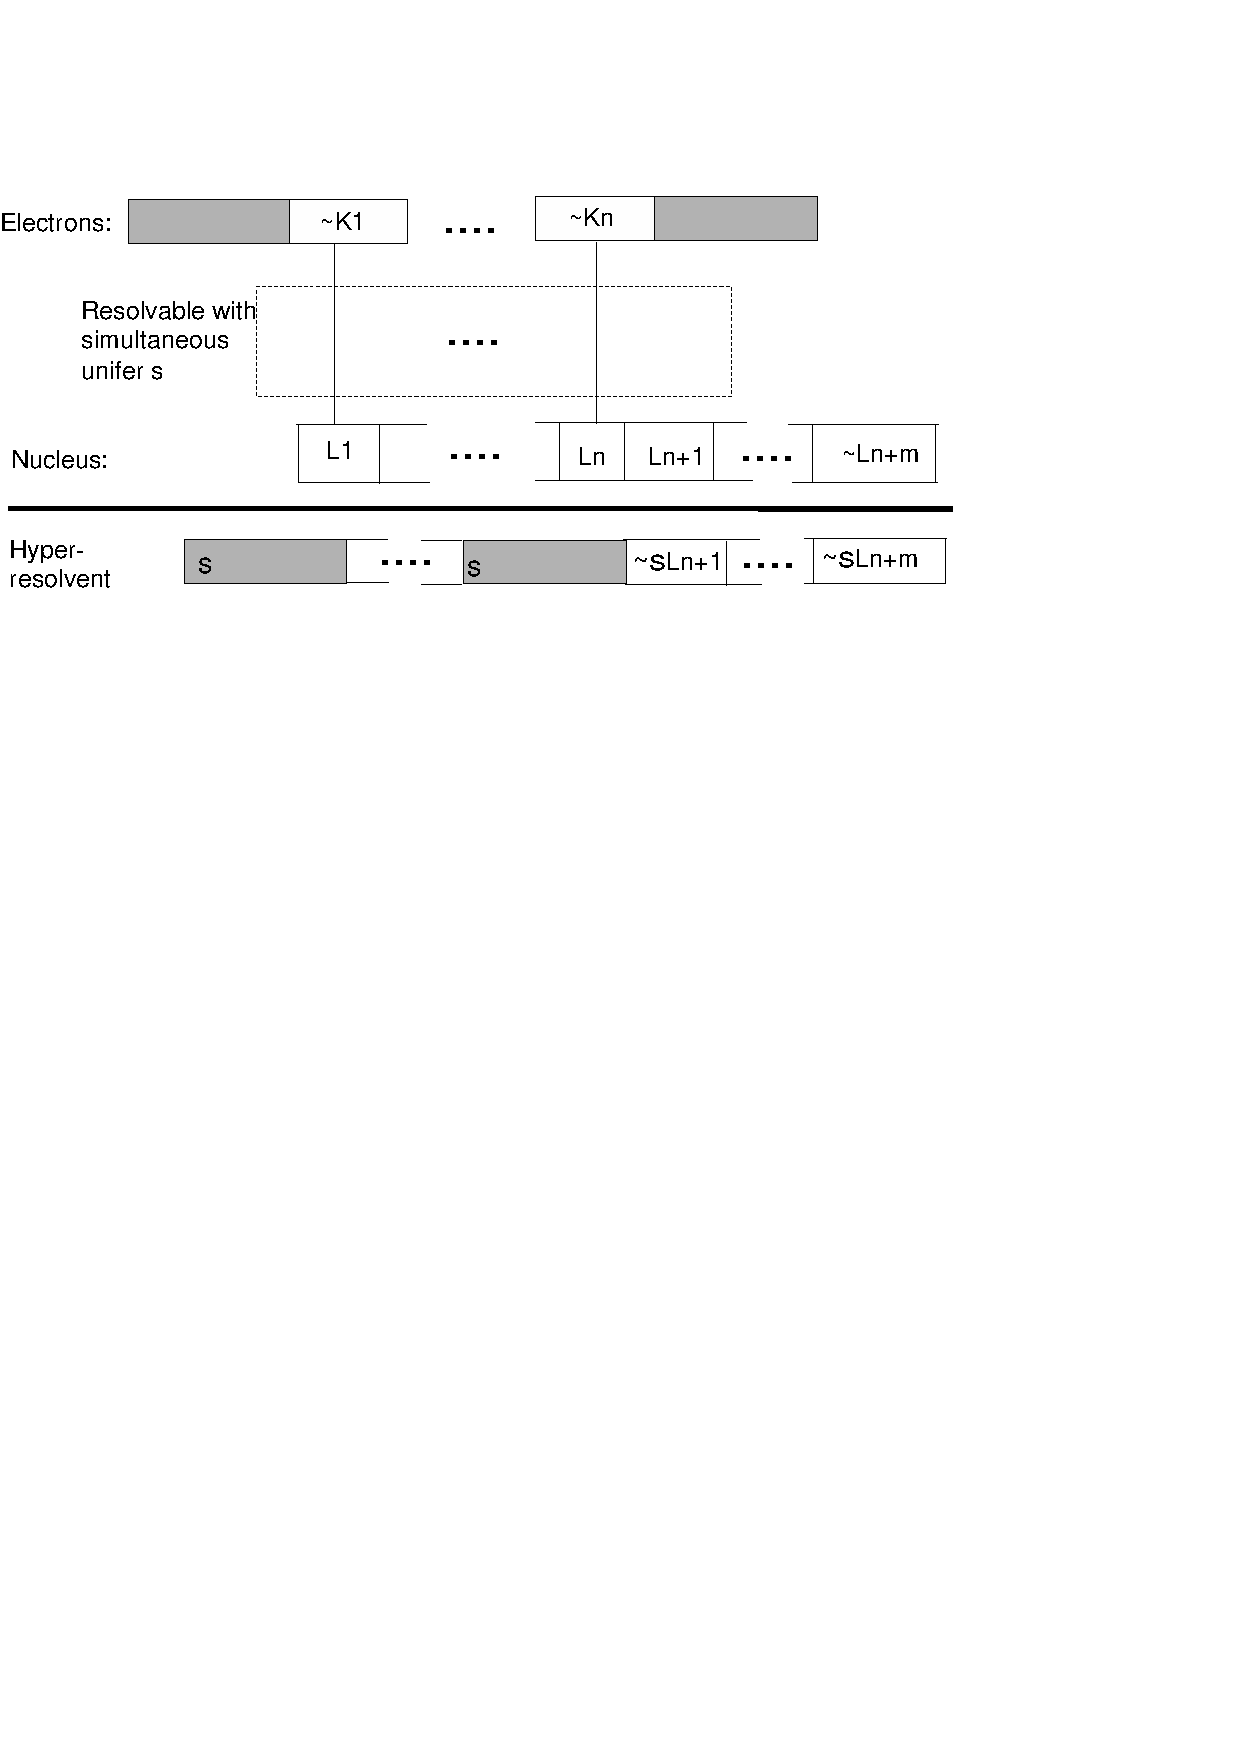
\includegraphics[width=\textwidth]{hyper-res.pdf}
    \caption{{hyper resolution のスキーム}}
    \label{fig:hyper-res}
  \end{center}
\end{figure}

図で nucleus とあるのは, 少なくとも一つの正のリテラルをもつ節である.
反駁可能な節集合にはこのような節が必ず存在する.
nucleus の個々の正のリテラルにつき, 負のリテラルのみを持つ節 electron が必要である.
やはり, 反駁可能な節集合にはこのような節が必ず存在する.
nucleus は全ての electron と「同時に」resolve されなければならない. 
結果として負のリテラルのみからなる節が, 導出節として得られる(図の hyper-resolvent).
この導出節は, 以降の hyper-resolution ステップで electron として使用することが出来る.

我々の反駁エンジンでは, フラグ neg-hyper-res が on の時に
使用される negative-hyper-resolution に相当する.

\subsection{Positive Hyper Resolution}

フラグ hyper-res が on の時に使用されるのは, これと dual な関係にある,
\textsl{positive} hyper resolution である. 
これは, 上で述べたスキームで, リテラルの 正/負 を逆にする事で得られ,
PI-resolution で,解釈 $I$ に含まれる各リテラルが否定記号を含む場合に
相当する.

否定の形で与えられる結論は, 通常負のリテラルのみを含むことが多いため,
negative hyper-resolution の electron として用いる事が出来るので,
結論から仮定へ向かっての, 後向き推論に適していると言える.
一方 positive hyper-resolution は, 仮定から結論へ向けての, 前向きの
推論が可能である. 

%%%%%%%%%%%%%%%%%%%%%%%%%%%%%
\section{Paramodulation}
\label{sec:paramod}

paramodulation は等号を扱うための推論ルールである. 
図~\ref{fig:paramod-rule} に paramodulation のスキームを示す.
図で, $l = r$ は \textbf{paramodulator} (正の等式リテラル), 
$f(t)$ は $t$ を副項に持つようなリテラル
である. $f(\sigma{r})$ は, その $t$ を $\sigma(r)$ で置き換えた項を
表すものとする.

\begin{figure}[htbp]
  \begin{center}
    $$
    \infer{
      \begin{array}{ll}
        \mbox{\textbf{paramodulant:}} &
        f(\sigma r), \sigma L_1,\cdots,\sigma L_n,\sigma M_1,\cdots,\sigma M_m
      \end{array}
      }
    {\begin{array}{l}
        l = r, L_1,\cdots,L_n \\
        f(t), M_1,\cdots,M_m
      \end{array}\hskip2cm\sigma は l と t の mgu
      }
    $$
    \caption{{paramodulation のスキーム}}
    \label{fig:paramod-rule}
  \end{center}
\end{figure}
図で, $sigma$ は, リテラル $f(t)$ の副項 $t$ と paramdulator の
左辺 $l$ との mgu(most general unifier) である ($\sigma l = t$).
paramodulant は $t$ を paramodulator の右辺に $sigma$ を適用した
もの($f(\sigma r)$) で置き換えることによって得られる.

%%%%%%%%%%%%%%%%%%%%%%%%%%%%%%%%%%%%%%%%%%%%%%%
\section{Demodulation}
\label{sec:demod}

demodulation は,導出された節に適用され,それに含まれるリテラルのアトムを
簡約化する.
すなわち,$l\rightarrow r$ の形をした demodulator があり,あるリテラル
$l$ が項 $t$ を副項として含む $P[t]$ の形をしているものとする.
このとき,$\sigma l = t$ となるような,変数置換があったときに,
$l$ を,$P[\sigma r]$ に書き換える.

demodulator として,$L = R$ という等式のリテラルのみからなる節が用いられる.
これを,項の書き換え規則として用いるためには,
等式の方向付けが必要である.
つまり,何らかの順序関係によって,等式の左右辺を方向付ける必要が
ある.反駁エンジンでは,この順序の判定に,単純な辞書式順と lrpo の 2種 を用意する.

\subsection{実行時のdemodulator判定}
\label{sec:dynamic-demodulator}

フラグ dynamic-demod が on の場合, 反駁エンジンは,
全ての equality ($\alpha = \beta$)を demodulator として使えるか
どうかを判定する.

フラグ dynamic-demod あるいは, dynamic-demod-all が on になっている
状況では, 必ずフラグ order-eq が on になっているはずである.
この時フラグ lrpo が on の場合には, 等式の向きつけの判定として
LRPO を,
そうでない場合は単純な重みと辞書式順による比較が行われる.
この結果等式の向きつけが行われるが, その
節が demodulator として使えるかどうかは, 次のような処理で
判定される.
なお検査の対象とする節は, 正の equality かつ単一節である.

\begin{enumerate}
\item 節のリテラル $l (\alpha = beta)$ に関して以下の判定を実行する:
  \begin{description}
  \item[フラグ lrpo が off の場合]
    \begin{enumerate}
    \item $\beta$ が $\alpha$ の副項であれば :normal とする
    \item 辞書式順の意味で 
      $\alpha > \beta$ かつ $vars(\alpha) \supseteq vars(\beta)$
      ならば,
      \begin{enumerate}
      \item フラグ dynamic-demod-all が on であれば OK とする
      \item dynamic-demod-all が off で $wt(\beta)\leq 1$ ならば
        OK とする
      \item それ以外の場合は NG とする
      \end{enumerate}
    \item フラグ dynamic-demod-lex-dep と dynamic-demod-all の
      両方が on のとき, $\alpha$ と $\beta$ が変数を除外すれば,
      構文的に同一の項である場合に ORDER-DEP とする.
    \item それ以外の場合は NG とする
    \end{enumerate}
  \item[フラグ lrpo が on の場合]
    \begin{enumerate}
    \item $l$ の等式の向きつけが正しく行われている場合, OK とする.
    \item フラグ dynamic-demod-lex-op が on の場合,
      $vars(\alpha)\supseteq vars(\beta)$ ORDER-DEP とする.
    \item それ以外の場合は NG とする
    \end{enumerate}
  \end{description}
\end{enumerate}

上の処理で, $vars(t)$ は, 項 $t$ に出現する変数の集合を意味する.

\subsection{Back Demdulation の実行}
\label{sec:back-demodulate}

back demodulation とは,導出された節が正の単一の equality 節
(一つの $\alpha = \beta$ の形のリテラルのみからなる節) で
あった場合に,それを demodulator として用いて,usable および
sos に含まれる全ての節に関して demodulation を実行するものである.

導出節が demodulator として適切なものかどうかの判定は,
導出節に対する前処理(第\ref{sec:pre-process}節
を参照)で行われている.

%%% Local Variables: 
%%% mode: latex
%%% TeX-master: t
%%% End: 


\newpage

% BIB %%%%%%%%%%%%%%%%%%%%%%%%%%%%%%%%%%%%%%%%%%%%%%%%%%%%%%
\begin{center}
\begin{thebibliography}{99}\itemsep=0pt

\bibitem{chang-lee} Chang, C. and Lee. R.C.,
  \textsl{Symbolic Logic and Mechanical Theorem Proving},
  Academic Press, 1973

\bibitem{ha} Joseph Goguen and Grant Malcolm, ``A Hidden Agenda'', in
  \emph{Theoretical Computer Science}, Vol.245 No.1, 2000, pp.55--101

\bibitem{otter} William McCune, ``\textsc{Otter3.0} Reference Manual
  and Guide'', Technical Report ANL-94/6, Argonne National Laboratory,
  1994, available at \texttt{http://www-unix.mcs.anl.gov/AR/otter/}

\bibitem{cafeobj} A.T.Nakagawa, T. Sawada, and K. Futatsugi,
  ``\textsl{CafeOBJ Manual}'', avaiable at 
  \texttt{ftp://ftp.sra.co.jp/lang/CafeOBJ/Manual/}

\bibitem{CafeRep} R\u{a}zvan Diaconescu and Kokichi Futatsugi,
  \textsf{CafeOBJ} \emph{Report}. World Scientific, 1998

\end{thebibliography}
\end{center}
\end{document}

